% ----------------------------- BASI DEL LINGUAGGIO ----------------------------------

\chapter{Basi del Linguaggio}

%TODO: allocazione dinamica della memoria? malloc, calloc, realloc? o in un altro capitolo?
%TODO: aggiungere gli pseudo random generators?
%TODO: volendo scrivere qualcosa riguardo il compilatore, il preprocessore, ecc..
%TODO: parlare del linker + immagini.

%TODO: C vs C++

%TODO: includere #include <iostream> negli esempi che lo usano.

% -------------------------- SECTION: INTRODUZIONE -----------------------------------

\section{Introduzione}

\enlargethispage{1\linewidth}

\textsf{\small Questa è una semplice e breve guida sul linguaggio C++. }\\

\textsf{\small Non insegna a programmare,
semplicemente è una collezione di frammenti di codice e spiegazioni delle sintassi
del linguaggio e alcune accortezze e good practices.}

\textsf{\small Questa è una guida per chi ha già familiarità con altri linguaggi di programmazione, come Java, C\# e vorrebbe avvicinarsi al C++.}\\

\textsf{\small Questa guida volge attorno alla versione C++17, ma vedremo anche alcuni concetti di C++20.
Mentre, l'ultima preview mostrata è stata quella del C++23.}\\

% -------------------------- SECTION: LINGUAGGIO -------------------------------------

\section{Linguaggio}

\textsf{\small Il C++ è un linguaggio di programmazione general purpose nato nel 1983 da Bjarne Stroustrup nei Bell Labs come evoluzione del C.}\\

\textsf{Il nome del linguaggio deriva dal C, ma con l'aggiunta dell'operatore ++ che nel C serve per incrementare di 1. Il che stava a significare che il C++ è come il C, ma migliore, ovvero come suo successore.}\\

% -------------------------- SECTION: PREPROCESSOR -----------------------------------

\newpage

\section{Preprocessor}

\textsf{\small Il \textbf{preprocessore} è composto da delle direttive che danno istruzioni al compilatore di preprocessare prima dell'effettiva compilazione.} \\

\textsf{\small Per esempio di includere una libreria standard del linguaggio.} \\

\textsf{\small Le direttive del preprocessore iniziano con il \textbf{\#}.} \\

\begin{lstlisting}
	// Con la direttiva \#include diciamo al preprocessore di includere questo file
	// che in questo caso si tratta della libreria standard per l'input ed output
	// del C++
	#include <iostream> 
\end{lstlisting}

% -------------------------- SECTION: COMPILATORE ------------------------------------

\section{Compilatore}

\textsf{\small Il C++ è un linguaggio di programmazione, di solito, implementato tramite un \textbf{compilatore} (un \emph{traduttore} che converte il \emph{codice sorgente} in \emph{codice macchina} object byte code) invece di un \textbf{interprete} (che esegue il direttamente il codice sorgente).} \\

%TODO: precompilatore, ecc..

% -------------------------- SECTION: LINKER -----------------------------------------

\section{Linker}

\textsf{\small Se il compilatore traduce il codice sorgente, il \textbf{linker} si occupa di risolvere le referenze ad altri files, per esempio all'inclusione di librerie standard del linguaggio. Quindi il linker linka i files che servono al tuo codice per essere eseguito al tuo codice (che dopo la compilazione sarà probabilmente diventato un .OBJ)} \\

%TODO: + immagini.

% -------------------------- SECTION: C VS C++ ---------------------------------------

\newpage

\section{C vs C++}

\begin{longtable}{|c|c|}
	\hline
	\textbf{C} & \textbf{C++} \\
	\hline
	\endhead
	%\endfoot
	\textsf{\small Sviluppato da Dennis Ritchie } & \textsf{\small Sviluppato da Bjarne Stroustrup } \\
	\textsf{\small tra gli anni 1969 e 1973 agli AT\&T Bell Labs.} & \textsf{\small tra il 1979 ed il 1983.} \\
	\hline
	\textsf{\small Non supporta il polimorfismo, incapsulazione,  } & \textsf{\small Supporta polimorfismo, incapsulazione } \\
	\textsf{\small ereditarietà il che significa che il C} & \textsf{\small ed ereditarietà il che significa} \\
	\textsf{\small non supporta la} & \textsf{\small  che è un linguaggio} \\
	\textsf{\small programmazione ad oggetti.} & \textsf{\small  di programmazione ad oggetti.} \\
	\hline
	\textsf{\small C è un sottoinsieme del C++.} & \textsf{\small Il C++ è un sovrainsieme del C.} \\
	\hline
	\textsf{\small Il C contiene 32 keywords.} & \textsf{\small Il C++ 63 keywords.} \\
	\hline
	\textsf{\small Il C supporta  } & \textsf{\small Il C++ è un ibrido, } \\
	\textsf{\small la programmazione } & \textsf{\small supporta sia la } \\
	\textsf{\small procedurale.} & \textsf{\small programmazione procedurale} \\
	\textsf{\small } & \textsf{\small sia i paradigmi della} \\
	\textsf{\small } & \textsf{\small programmazione ad oggetti.} \\
	\hline
	\textsf{\small Dati e funzioni sono separati} & \textsf{\small Dati e funzioni sono} \\
	\textsf{\small perché è un linguaggio} & \textsf{\small incapsulati in forma} \\
	\textsf{\small di programmazione procedurale.} & \textsf{\small di un oggetto.} \\
	\hline
	\textsf{\small Non supporta } & \textsf{\small I dati sono incapsulati } \\
	\textsf{\small l'information hiding.} & \textsf{\small per garantire che } \\
	\textsf{\small } & \textsf{\small vengano usati come inteso.} \\
	\hline
	\textsf{\small Tipi incorporati sono supportati} & \textsf{\small Tipi incorporati e tipi definiti} \\
	\textsf{\small dal C. (typedef).} & \textsf{\small dall'utente sono supportati.} \\
	\hline
	\textsf{\small Basata sulle funzioni perché} & \textsf{\small Basata sugli oggetti perché} \\
	\textsf{\small è un linguaggio procedurale.} & \textsf{\small è un linguaggio ad oggetti.} \\
	\hline
	\textsf{\small L'overloading delle funzioni e} & \textsf{\small L'overloading delle funzioni e} \\
	\textsf{\small degli operatori non è supportato.} & \textsf{\small degli operatori è supportato.} \\
	\hline
	\textsf{\small Non si possono definire funzioni} & \textsf{\small Si possono definire funzioni} \\
	\textsf{\small dentro le strutture.} & \textsf{\small dentro le strutture.} \\
	\hline
	\textsf{\small Namespaces non esistono in C.} & \textsf{\small Namespace sono presenti in C++.} \\
	\textsf{\small File header di input ed output} & \textsf{\small File header di input ed output} \\
	\textsf{\small in C è stdio.h.} & \textsf{\small in C++ è iostream.} \\
	\hline
	\textsf{\small Le variabili di referenza non sono supportate.} & \textsf{\small Le variabili di referenza sono supportate.} \\
	\hline
	\textsf{\small Le funzioni virtual e} & \textsf{\small Le funzioni virtual e} \\
	\textsf{\small friends non sono supportate.} & \textsf{\small friends sono supportate.} \\
	\hline
	\textsf{\small Non supporta l'ereditarietà.} & \textsf{\small Supporta l'ereditarietà.} \\
	\hline
	\textsf{\small Si concentra sulle funzioni} & \textsf{\small Si concentra sui dati} \\
	\textsf{\small più che sui dati.} & \textsf{\small più che sulle funzioni.} \\
	\hline
	\textsf{\small Fornisce malloc(), calloc(), realloc()} & \textsf{\small Fornisce gli operatori new e delete (e altro)} \\
	\textsf{\small e free() per } & \textsf{\small per  } \\
	\textsf{\small l'allocazione/deallocazione dinamica} & \textsf{\small l'allocazione/deallocazione dinamica} \\
	\textsf{\small  della memoria.} & \textsf{\small della memoria.} \\
	\hline
	\textsf{\small Supporto diretto per occuparsi} & \textsf{\small Supporto diretto per occuparsi} \\
	\textsf{\small delle eccezioni non è supportato.} & \textsf{\small delle eccezioni è supportato.} \\
	\hline
	\textsf{\small scanf() e printf() sono usate} & \textsf{\small cin e cout sono usate} \\
	\textsf{\small per l'input/output in C.} & \textsf{\small per l'input/output in C++.} \\
	\hline
	\textsf{\small Le strutture in C non hanno} & \textsf{\small Le strutture in C++ hanno} \\
	\textsf{\small modificatori d'accesso.} & \textsf{\small modificatori d'accesso.} \\
	\hline
\end{longtable}

% -------------------------- SECTION: TIPI DI DATI -----------------------------------

\newpage

\section{Tipi di Dati}

%\verb!C++! % modo per scrivere C++

\textsf{\small Il C++ possiede diverse tipologie di memorizzazione dei dati: }\\

\begin{figure}[ht]
	\centering
	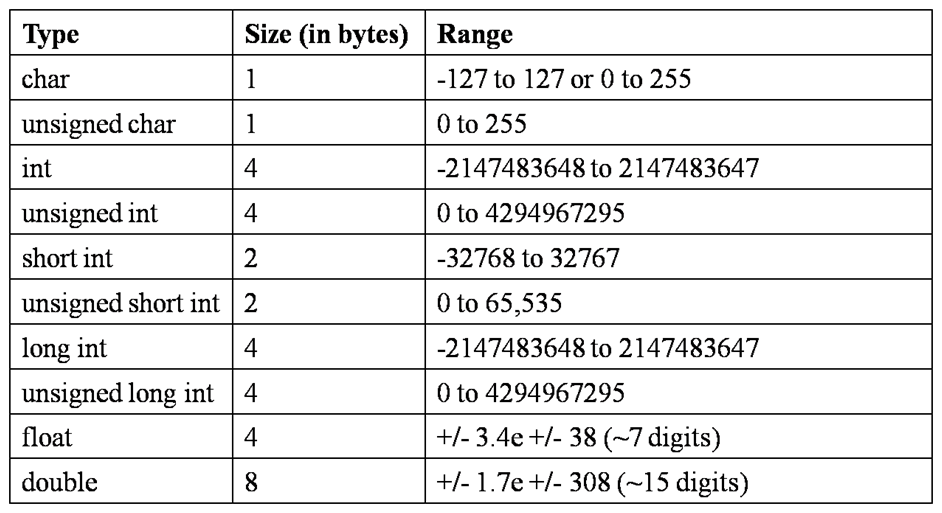
\includegraphics[width=1\textwidth, height=1\textheight, keepaspectratio]{./imgs/data_types_table.png}
	\caption{Tabelle dei tipi}
	\label{fig:data_types}
\end{figure}

\textsf{\small E dei wrappers sui tipi \textbf{unsigned} (ovvero senza segno, ovvero sempre e solo positivi), come: }\\

\begin{tabular}{cc}
	\color{myblue2}size\_t & corrisponde ad unsigned int \\
	\color{myblue2}uint8\_t & unsigned char \\
	\color{myblue2}uint16\_t & unsigned int  \\
	\color{myblue2}uint32\_t & unsigned long \\ 
\end{tabular} \\

\textsf{\small E altri tipi di dati per lavorare sui caratteri e sulle stringhe: }\\

\begin{tabular}{cc}
	\color{myblue2}string & (includere string) \\
	\color{myblue2}wchar\_t & wide char (per caratteri più grandi di 255) \\
\end{tabular}

\break

\textsf{\small Altri tipi di dati: } \\

\begin{tabular}{cc} %TODO: aggiungerne altri volendo.
	\color{myblue2}bool & Un booleano : o 0, ovvero FALSO/OFF o 1, ovvero TRUE/ON \\
	\color{myblue2}std::byte & 8 bit (definito in <cstddef> header file) \\
	\color{myblue2}register &  un registro\\ 
	\color{myblue2} auto &  trova la tipologia automaticamente\\
\end{tabular}\\

\textsf{\small Esistono anche altri tipi, ma quelli qui riportati sono tra i più comuni.}\\

\subsection{Cast}

\textsf{\small \textbf{Definizione: } Il \textbf{Cast} è un'operazione che permette di cambiare la tipologia di una variabile o di una determinata operazione matematica.} 

\textsf{\small Ovviamente, questa operazione potrebbe portare ad una perdita di dati, in particolare, quando facciamo un cast da una tipologia più grande (che occupa più spazio, più bits) ad una più piccola (che occupa meno spazio, meno bits) perché quella piccola non ha lo stesso spazio di immagazzinamento di quella grande.} 

\textsf{\small Per esempio se si fa un cast da una tipologia a 32 bit ad una a 8 bit, ovviamente si perderanno dei dati, perchè quella da 8 non può contenere gli stessi dati di una da 32.} \\

\textsf{\small Per fare un cast bisogna mettere, prima dell'operazione, tra parentesi la tipologia a cui si vuole castare. Esempio: (float) 5 / 2 = 3.5} \\

\begin{lstlisting}
	// Primo esempio:
	
	int a = 7, b = 2;
	float c;
	
	c = a / b; // Output : 3
	
	c = (float) a / b; // Output : 3.5
	
	// Secondo esempio:
	
	double d = 36.9;
	float f = 22.2;
	int x;
	
	x = (int) d; // Output : 36
	x = (int) f; // Output : 22
	
	// Ovviamente una variabile intera non può contenere i dati delle variabili con la virgola e quindi le informazioni sulla virgola vengono perse.
\end{lstlisting}

\textsf{\small Questo è un cast semplice, ci sono altre forme di cast un po' più complesse che vedremo in un altro capitolo.} \\

% -------------------------- SECTION: COSTANTI ---------------------------------------

\newpage

\section{Costanti}

\textsf{\small Una costante è un valore che non cambia mai.}\\

\textsf{\small Ci sono diversi tipi di costanti e con significato diverso, per esempio \color{myblue2} cost \normalcolor e \color{myblue2} constexpr. \normalcolor}\\

\subsection{const vs constexpr}

\begin{tabular}{|c|c|}
	\hline
	\textbf{const} & \textbf{constexpr} \\
	\hline
	\textsf{\small può essere composta da altre variabili a run-time} & \textsf{\small deve essere conosciuta a compile-time} \\
	%\hline
	\textsf{\small può essere usata solo per } & \textsf{\small può essere usata sia per member } \\
	\textsf{\small non-static member functions} & \textsf{\small e non-member functions} \\
	\textsf{\small } & \textsf{\small e anche costruttori} \\
	\hline
\end{tabular}\break

\subsection{static}

\subsubsection{Variabili statiche}

\textsf{\small Viene allocata per l'intera durata del programma. Anche se la funzione è chiamata molteplici volte, lo spazio allocato per la variabile statica è allocato una volta sola.} \\

\subsubsection{Membri statici delle classi} %TODO: sistemare questa parte.

\centering\textbf{Istanze delle classi come statiche} \\

\textsf{\small I distruttori (funzioni che rimuovo l'allocazione di memoria di un oggetto classe) vengono invocati soltanto dopo la fine del main (funzione principale da cui parte tutto il programma).} \break

\centering\textbf{Funzioni statiche in una classe} \\

\textsf{\small Queste possono soltanto accedere a dati statici o altre funzioni statiche.} \\

\subsection{static const}

\textsf{\small Per quanto riguarda \color{myblue2} static const \normalcolor possono ottenere un valore a compile time o a runtime, proprio come \color{myblue2} const, \normalcolor ma solo accessibili nella data funzione/classe.}\\

\subsection{static constexpr}

%TODO: scrivere qualcosa su static constexpr

\begin{figure}[ht]
	\centering
	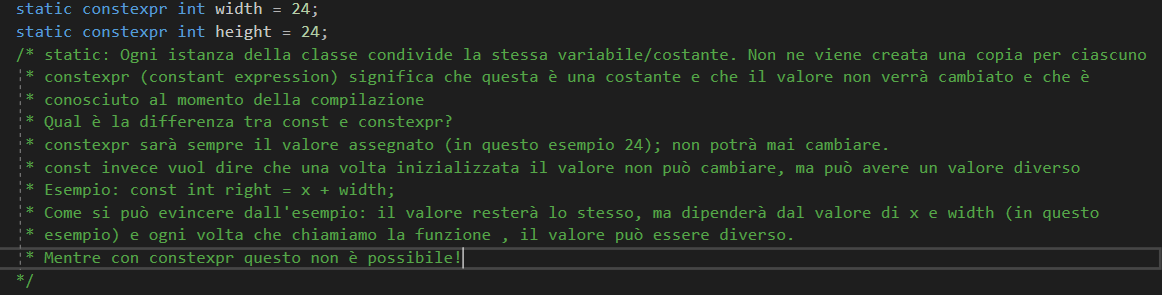
\includegraphics[width=1.2\textwidth, height=1.2\textheight, keepaspectratio]{./imgs/constexpr_e_const_differenze.png}
	\caption{Tipi di costanti}
	\label{fig:constants}
\end{figure}

% -------------------------- SECTION: ARRAYS E MATRICI -------------------------------

\section{Arrays e Matrici}

\subsection{Arrays}

\textsf{\small \textbf{Definizione: } Gli array sono dei contenitori di dati, una collezione di dati dello stesso tipo.} \\

\textsf{\small Il primo elemento di un array, come qualsiasi altra cosa in informatica è l'elemento 0, non l'elemento 1.}\\

\textsf{\small Quindi l'elemento di indice 0 è il primo elemento, quello di indice 1 è il secondo, quello di indice 2 è il terzo e cosi via..} \\

\begin{lstlisting}[language=C++]
	// tipologia nomeDelArray[ spazioOccupato ];
	
	double dArray[3];
	
	// Qui potremmo usare un loop per definire questi elementi, 
	// ma li vedremo dopo.
	dArray[0] = 12.4;
	dArray[1] = 37.9;
	dArray[2] = 19.1;
	
	// Possiamo assegnarli anche quando definiamo l'array.
	int array[5] = {7, 9, 12, 4, 11};
	
	// Potremmo anche non definire il size (spazio dell'array).
	int array2[] = {3, 6, 9};
	
	// Ma è raccomandabile usare dei contenitori come: std::vector 
	// oppure una lista.
	// Oppure dei puntatori.
	// Oppure dei smart pointers.
\end{lstlisting}

\subsection{Matrici}

\textsf{\small \textbf{Definizione: } Le matrici sono degli arrays organizzati su righe e colonne. Questo concetto è per una matrice di 2-dimensioni. La si può pensare proprio come una tabella, formata da righe e da colonne.} \\

\begin{lstlisting}
	#include <iostream> 
	
	// <iostream> è un file di intestazione (header file) della libreria standard per poter lavorare sull'input e sull'output.
	
	// tipologia nome\_matrice [righe][colonne];
	
	int matrix[3][3] = {{1,2,3}, {4,5,6}, {7,8,9}}
	
	for(int i = 0; i < 3; i++){
		for(int j = 0; j < 3; j++){
			std::cout << "elemento di riga " << i << " e colonna " << j << matrix[i][j] << std::endl;
		}
	}
\end{lstlisting}

\textsf{\small Ovviamente, come in matematica, è possibile eseguire varie operazioni sulle matrici, come: trasposizione, moltiplicazione, somma, sottrazione, ecc..(ma che qui non mostrerò).} \\ 

% -------------------------- SECTION: OPERATORI ARITMETICI ---------------------------

\section{Operatori Aritmetici}

\textsf{\small \textbf{Definizione: } Gli operatori aritmetici permettono di eseguire qualsiasi operazione aritmetica.} \\

\begin{itemize}
	\item \textsf{\small \textbf{+} : somma.}
	\item \textsf{\small \textbf{-} : sottrazione.}
	\item \textsf{\small \textbf{*} : moltiplicazione.}
	\item \textsf{\small \textbf{/} : divisione.}
	\item \textsf{\small \textbf{\%} : modulo, restituisce il resto della divisione.}
\end{itemize}

\begin{lstlisting}
	int a = 8, b = 3;
	
	a + b; // Output : 11
	
	a - b; // Output : 5
	
	a * b; // Output : 24
	
	a / b; // Output : 2
	
	a % b; // Output : 2 (resto della divisione)
	
\end{lstlisting}

% -------------------------- SECTION: OPERATORI RELAZIONALI --------------------------

\section{Operatori Relazionali}

\textsf{\small \textbf{Definizione: } Gli operatori relazionali servono per controllare la relazione tra due operandi. } \\

\begin{itemize}
	\item \textsf{\small \textbf{==} : per l'equivalenza; controllare se due operandi sono uguali.}
	\item \textsf{\small \textbf{!=} : per controllare se due operandi non sono equivalenti.}
	\item \textsf{\small \textbf{>} : per controllare se un operando è maggiore dell'altro}
	\item \textsf{\small \textbf{>=} : per controllare se un operando è maggiore o uguale all'altro.}
	\item \textsf{\small \textbf{<} : per controllare se un operando è minore di dell'altro.}
	\item \textsf{\small \textbf{<=} : per controllare se un operando è minore o uguale all'altro.}
\end{itemize}

\begin{lstlisting}
	int x = 5, y = 3;
	x == y // Output : FALSE
	x != y // Output : TRUE
	x > y // Output : TRUE
	x >= y // Output : TRUE
	x < y // Output : FALSE
	x <= y // Output : FALSE
	
\end{lstlisting}

% -------------------------- SECTION: OPERATORI BITWISE ------------------------------

\section{Operatori Bitwise}

\textsf{\small \textbf{Definizione: } Gli operatori bitwise servono per lavorare sui singolo bits di dati.} \\

\begin{itemize}
	\item \textsf{\small \textbf{\& (bitwise AND)} : permette di fare un AND bit a bit sui due operandi. Il risultato è 1 soltanto se entrambi sono 1.}
	\item \textsf{\small \textbf{| (bitwise OR)} : permette di fare un OR bit a bit su ogni bit dei due operandi. Il risultato è 1 se almeno uno dei due bits è a 1.}
	\item \textsf{\small \textbf{\^  (bitwise XOR)} : permette di fare uno XOR bit a bit su ogni bit dei due operandi. Il risultato è 1 se i due bits sono differenti.}
	\item \textsf{\small \textbf{$<<$ (left shift)} : prende due numeri. Shifta a sinistra i bits del primo operando, il secondo operando decide di quanti bits si deve shiftare il primo.}
	\item \textsf{\small \textbf{$>>$ (right shift)} : prende due numeri. Shifta a destra i bits del primo operando, il secondo operando decide di quanti bits si deve shiftare il primo.}
	\item \textsf{\small \textbf{\~ (bitwise NOT)} : prende un numero ed inverte tutti i bits.}
\end{itemize}

\begin{lstlisting}
	// a = 5 in binario è 00000101, b = 9 in binario è 00001001
	int a = 5, b = 9;
	
	a & b; // Output : 00000001
	
	a | b; // Output : 00001101
	
	a ^ b; // Output : 00001100
	
	~a; // Output : 11111010
	
	b << 1; // Output : 00010010
	
	b >> 1; // Output : 00000100
	
	
\end{lstlisting}

% ---------- SECTION: OPERATORI DI ASSEGNAMENTO E OPERATORI UNARI --------------------

\section{Operatori di Assegnamento e Operatori Unari}

\subsection{Operatori di Assegnamento}

\textsf{\small \textbf{Definizione: } Gli operatori di assegnamento sono usati per assegnare un valore alle variabili.} \\

\begin{itemize}
	\item \textsf{\small \textbf{=} : Operatore di assegnamento di un valore ad una variabile.}
	\item \textsf{\small \textbf{+=} : Combinazione di = e +, aggiunge l'operando di destra a quello di sinistra e lo assegna a quello di sinistra.}
	\item \textsf{\small \textbf{-=} : Combinazione di = e -, sottrae l'operando di destra a quello di sinistra e lo assegna a quello di sinistra.}
	\item \textsf{\small \textbf{*=} : Combinazione di = e *, moltiplica l'operando di destra a quello di sinistra e lo assegna a quello di sinistra.}
	\item \textsf{\small \textbf{/=} : Combinazione di = e /, divide l'operando di destra a quello di sinistra e lo assegna a quello di sinistra.}
	\item \textsf{\small \textbf{\%=} : Combinazione di = e \%, ottiene il resto dall'operando di destra a quello di sinistra e lo assegna a quello di sinistra.}
	\item \textsf{\small \textbf{$<<$=} : Combinazione di = e $<<$, left shifta l'operando di destra a quello di sinistra e lo assegna a quello di sinistra.}
	\item \textsf{\small \textbf{$>>$=} : Combinazione di = e $>>$, right shifta l'operando di destra a quello di sinistra e lo assegna a quello di sinistra.}
	\item \textsf{\small \textbf{\&=} : Combinazione di = e \&, bitwise AND sull'operando di destra a quello di sinistra e lo assegna a quello di sinistra.}
	\item \textsf{\small \textbf{\^ =} : Combinazione di = e \^, bitwise XOR sull'operando di destra a quello di sinistra e lo assegna a quello di sinistra.}
	\item \textsf{\small \textbf{|=} : Combinazione di = e |, bitwise OR sull'operando di destra a quello di sinistra e lo assegna a quello di sinistra.}
	\item \textsf{\small \textbf{$<>$=} : Bitwise shift left/right assignment} 
\end{itemize}

\begin{lstlisting}
	int x = 5; // = è un operatore di assegnamento.
	int y;
	
	y += 3; // += è un operatore di assegnamento ed è la combinazione dell'operatore = e l'operatore +. Scrivere y += 3; è identico a scrivere y = y + 3; (ovvero y è uguale a se stesso + 3).
	
	y -= 2; // identico a y = y - 2;
	
	y *= 4; // identico a y = y * 4; (* è un per, oppure viene usato nei puntatori)
	
	y /= 6; // identico a y = y / 6;
	
\end{lstlisting}

\subsection{Operatori Unari}

\textsf{\small \textbf{Definizione: } Gli operatori unari operano su un operando per produrre un nuovo valore.} \\

\begin{itemize}
	\item \textsf{\small \textbf{-} : nega il valore dell'operando.}
	\item \textsf{\small \textbf{++nome\_variabile} : Incremento di 1 prefix, prima incrementa l'operando prima che venga eseguito.}
	\item \textsf{\small \textbf{nome\_variabile++} : Incremento postfix, il valore verrà incrementato dopo che è stato usato.}
	\item \textsf{\small \textbf{- -nome\_variabile} : Decremento di 1 prefix, decrementa l'operando prima che venga usato. }
	\item \textsf{\small \textbf{nome\_variabile- -} : Decremento postfix, il valore verrà decrementato dopo che è stato usato.}
	\item \textsf{\small \textbf{\&nome\_variabile} : prima di una variabile, restituisce l'indirizzo di memoria della variabile in questione. In questo caso, NON è l'operatore bitwise AND \&.}
	\item \textsf{\small \textbf{!nome\_variabile} : operatore not, inverte lo stato logico dell'operando. Se è TRUE allora lo modifica in FALSE, se è FALSE allora diventa TRUE.}
\end{itemize}

\begin{lstlisting}
	int x = 3;
	
	-x; // l'operatore - nega il valore dell'operando.
	
	++x; // identico a scrivere x = x + 1; Questo è chiamato incremento prefisso, perché: in questo modo il valore dell'operando verrà alterato prima che venga usato.
	
	x++; // identico a scrivere x = x + 1; L'operatore ++ incrementa di 1 il valore della variabile in questione. Questo è chiamato incremento postfisso perché: in questo modo il valore verrà modificato dopo che è stato usato.
	
	--x; // identico a scrivere x = x - 1; Come per il ++ questo è un decremento prefisso.
	
	x--; // identico a scrivere x = x - 1; Decrementa di 1 il valore della variabile in questione. Decremento post fisso.
	
	&x; // l'operatore \&, prima di una variabile, restituisce l'indirizzo di memoria in cui la variabile risiede.
	
	bool y = true;
	
	!y; // Output : y è false;  l'operatore ! (not) inverte lo stato logico dell'operando.
	
\end{lstlisting}

% -------------------------- SECTION: OPERATORI LOGICI -------------------------------

\section{Operatori Logici}

\textsf{\small \textbf{Definizione: } Gli operatori logici servono per combinare due o più condizioni. Il risultato di un'operazione degli operatori logici è un booleano TRUE (VERO) o FALSE (FALSO).} \\

\begin{itemize}
	\item \textsf{\small \textbf{\&\& (logical AND)} : restituisce vero se tutte le condizioni sono vere.}
	\item \textsf{\small \textbf{|| (logical OR)} : restituisce vero se almeno una delle condizioni è vera.}
	\item \textsf{\small \textbf{! (logical NOT)} : restituisce vero se la condizione è falsa e restituisce falso se la condizione è vera.}
	\item \textsf{\small \textbf{!~} : Logical negation/bitwise complement} 
\end{itemize}

\begin{lstlisting}
	int x = 3, y = 6, z = 9;
	
	(x > y) || (y != z); // Output : TRUE, perché anche se x > y è FALSA, y != z è VERA.
	
	(y > x) && (y < z); // Output : TRUE perché entrambe sono vere.
	
	!(x > 7); // Output : TRUE, perché x non è maggiore di 7, quindi è falsa, ma il not inverte e quindi essendo la condizione falsa, il not la inverte in VERA.
	
\end{lstlisting}

% -------------------------- SECTION: ALTRI OPERATORI --------------------------------

\section{Altri Operatori}

\textsf{\small Ci sono altri operatori come: } \\

\begin{itemize}
	\item \textsf{\small \textbf{sizeof} : è usato per ottenere lo spazio che occupa una variabile.}
	\item \textsf{\small \textbf{,} : la virgola è usata sia come operatore che come separatore. valuta il primo operando e cancella il risultato, valuta il secondo operando e restituisce il suo valore.}
	\item \textsf{\small \textbf{Operatore Condizionale/Ternario} : condizione ? se vero esegui questo : se falso esegui questo.}
\end{itemize}

\begin{lstlisting}
	sizeof(char); // Output : 1
	sizeof(int); // Output : 4
	sizeof(float); // Output : 4
	sizeof(double); // Output : 8
	
	int a = 0;
	double d = 3.69;
	
	sizeof(a); // Output : 4
	sizeof(d); // Output : 4
	
	sizeof(a + d); // Output : 8
	
	int y = 2, x = 3; // Output : equivalente a int y = 2; int x = 3;
	
	x >= 0 ? "x è maggiore o uguale a 0" : "x è minore di 0"; // Output : "x è maggiore o uguale a 0".
\end{lstlisting}

% -------------------------- SECTION: IF STATEMENTS ----------------------------------

\newpage

\section{Condizione If}

\subsection{If|else if|else}

\textsf{\small \textbf{Definizione:} L'If statement permette di decidere se un certo blocco di codice verrà eseguito o no.} \\

\textsf{\small L'else statement permette di eseguire un altro blocco di codice, casomai la condizione sia falsa.} \\

\textsf{\small else if(condizione) statement permette di fare un'ulteriore controllo dopo al primo if statement. } \\

\subsection{Operatore Ternario}

\textsf{\small Un altro modo per valutare una condizione ed eseguire un codice è attraverso l'operatore ternario: condizione ? se è vera esegui questo : altrimenti esegui questo.} \\

\textsf{\small L'unica differenza con l'if è che si può eseguire una sola riga di codice sia nel caso la condizione sia vera sia falsa.} \\

\begin{lstlisting}
	if(condizione)
	{
		// Se (if) la condizione è vera esegui questo blocco di codide.
	} else {
		// Altrimenti (else) esegui questo blocco di codice.
	}

	// Esempio: Cerchiamo il valore maggiore.
	int x = 5, y = 3;
	
	if(x > y)
	{
		std::cout << "x è maggiore di y" << std::endl;
	} 
	else if(x == y){
		std::cout << "x ed y sono uguali" << std::endl;
	}
	else {
		std::cout << "x è minore di y" << std::endl;
	}

	// Qui invece cerchiamo il valore minore.
	int a = 8, b = 7;
	int min;
	
	min = a < b ? a : b;
	
	std::cout << "Il valore minimo è: " << min << std::endl;
\end{lstlisting}

\textsf{\small Se la riga da eseguire è 1 sola, allora si possono anche omettere le parentesi graffe.} \\

% -------------------------- SECTION: SWITCH -----------------------------------------

\section{Switch}

\subsection{Switch|Cases|Break}

\textsf{\small \textbf{Definizione: } Gli switch statements valutano una data espressione ed in base al valore di quella espressione, eseguono un determinato blocco di codice.} \\

\textsf{\small Le possibili espressioni che si possono mettere nello switch sono: }

\begin{itemize}
	\item \textsf{\small Un numero intero, \color{myblue2}int}
	\item \textsf{\small Un enumeratore, \color{myblue2}enum}
	\item \textsf{\small Un carattere, \color{myblue2}char \normalcolor che è un piccolo intero tra -128 e + 127.}
\end{itemize}

\textsf{\small Le varie scelte sono indicate nel \textbf{case}.} \\

\textsf{\small I cases son tutti collegati fra loro e quindi per far si che solo un blocco di codice venga eseguito utilizziamo la keyword \textbf{break} per poter uscire dallo switch una volta che il codice è stato eseguito.} 

\textsf{\small Se non mettessimo il \textbf{break} allora una volta eseguito un case, il codice che è sequenziale, eseguirebbe il case sotto. Possiamo evitare di metterlo se vogliamo che alcuni case eseguino lo stesso codice.} \\

\subsection{Default Case}

\textsf{\small Infine c'è un case \textbf{default} nel caso che il valore valutato non sia presente tra i case. Questo case è opzionale, quindi si può anche non includere.}

\textsf{\small Per il \textbf{default} non serve il \textbf{break} perchè è comunque l'ultimo case, però volendo lo si può sempre mettere.} \\

\begin{lstlisting}
	int scelta = 3;
	
	switch(scelta){
		case 1:
			std::cout << "Scelta: 1" << std::endl;
			// Blocco di codice per il case 1.
			break;
		case 2:
			std::cout << "Scelta: 2" << std::endl;
			// Blocco di codice per il case 2.
			break;
		case 3:
			std::cout << "Scelta: 3" << std::endl;
			// Blocco di codice per il case 3.
			break;
		default:
			std::cout << "Nessuna scelta o scelta non prevista." << std::endl;
			// Blocco di codice per il default case.
			break;
	}
\end{lstlisting}

% -------------------------- SECTION: LOOPS ------------------------------------------

\newpage

\section{Loops}

\textsf{\small \textbf{Definizione: } I loops (cicli) ci permettono di ripetere un dato blocco di codice per un determinato o indeterminato numero di volte.} \\

\subsection{While}

\textsf{\small I while loops ci permettono di eseguire un ciclo quando non conosciamo esattamente il numero di iterazioni. } \\

\textsf{\small La condizione del while viene valutata, se possibile entra dentro al loop altrimenti lo salta ed esegue il codice dopo.}

\textsf{\small Ad ogni iterazione la condizione viene controllata, se vera il ciclo continua, se falsa il ciclo viene interrotto.} \\

\begin{lstlisting}
	while(condizione){
		// Blocco di codice da eseguire.
	}

	int x = 3;
	
	while(x < 5){
		std::cout << "Ciao per la " << x << "a volta" << std::endl;
		x++; // indentico a x = x + 1
	}
\end{lstlisting}

\subsection{Do-While}

\textsf{\small Nel Do while rispetto al singolo while, si entra almeno una volta all'interno del ciclo, poi come nel while viene controllata la condizione e se vera il ciclo continua altrimenti verrà interrotto.} \\

\begin{lstlisting}
	do{
		// Blocco di codice da eseguire.
	}while(condizione); // da notare il ; dopo il while.

	int x = 2;
	
	do{
		std::cout << "Hello World!" << std::endl;
		x++;
	}while(x < 1);
\end{lstlisting}

\subsection{Continue}

\textsf{\small La keyword \textbf{continue} è simile alla keyword \textbf{break}, ma invece di terminare l'esecuzione (del loop, dello switch, ecc..) , passa alla prossima iterazione del loop.}\\

\begin{lstlisting}
	int a = 5;
	do {
		if(a == 10){
			a++;
			continue;
		}
		std::cout << "Valore di a: " << a << std::endl;
		a++;
	} while( a < 20);
\end{lstlisting}

\subsection{goto}

\textsf{\small La keyword \textbf{goto} permette di fare un salto incondizionato verso una label (etichetta).}

\textsf{\small Potrebbe essere utile per uscire dai cicli annidati (nested loops).}

\textsf{\small L'uso del \textbf{goto} è scoraggiato ed è considerato una \emph{bad practice} perché porta a quello che è definito \emph{spaghetti code}, ovvero ad un codice destrutturato e difficile da mantenere.} \\

\begin{lstlisting}
	int a = 10;
	
	LOOP:do {
		if( a == 15) {
			// skip the iteration.
			a = a + 1;
			goto LOOP;
		}
		cout << "value of a: " << a << endl;
		a = a + 1;
	} 
	while( a < 20 );
\end{lstlisting}

\subsection{For}

\textsf{\small Il for loop è composto da tre parti: l'inizializzazione della variabile contatore, la condizione, ed aggiornamento della variabile contatore. }

\textsf{\small A differenza del while loop, in questo conosciamo già a priori quanti cicli faremo.}

\textsf{\small Ad ogni iterazione del ciclo, la variabile contatore viene aggiornata.} \\

\begin{lstlisting}
	for(inizializzazione; condizione; aggiornamento variabile){
		// Codice da eseguire.
	}

	int n = 4;
	
	for(int i = 0; i < n; i++){
		// Codice da eseguire
	}
\end{lstlisting}

\subsection{Foreach}

%TODO: aggiungere la ref ai for each

\textsf{\small Questo loop è un po' più complicato e si avvale degli iteratori che verrano spiegati più avanti in un altro capitolo.} %\ref{}}

\textsf{\small È definito nel file di intestazione \textbf{\#include <algorithm>}.} \\

\subsection{Cicli annidati}

\textsf{\small Si può inserire un loop dentro ad un altro loop (cicli annidati o nested loops).} \\

\subsection{Cicli Infiniti}

\textsf{\small Bisogna fare attenzione a non creare cicli infiniti, che come dice la parola vanno ad oltranza, rallentano e bloccano il programma.}\\

\begin{lstlisting}
	for( ; ; ){
		std::cout << "Loop Infinito" << std::endl;
	}
\end{lstlisting}

% -------------------------- SECTION: ENUMS ------------------------------------------

\section{Enumeratori}

\textsf{\small \textbf{Definizione: } Gli enumeratori sono dei tipi di dati definiti dagli utenti ed usati per assegnare nomi a delle costati intere, il che rende il codice semplice da leggere.}

\textsf{\small Il primo elemento di un enum è di indice 0, ammeno che non lo si cambi, se lo si cambia, di conseguenza, cambiano anche tutti gli altri sotto.} \\

\begin{lstlisting}
	enum Days {Lunedi, Martedi, Mercoledi, Giovedi, Venerdi, Sabato, Domenica};
	Days day = Venerdi;
	
	if(day == Venerdi){
		std::cout << "Oggi è venerdi!" << std::endl;
	}
	
	enum Year {
		GENNAIO = 1,
		FEBBRAIO,
		MARZO,
		APRILE,
		MAGGIO,
		GIUGNO,
		LUGLIO,
		AGOSTO,
		SETTEMBRE,
		OTTOBRE,
		NOVEMBRE,
		DICEMBRE
	};

	Year mese = FEBBRAIO;
	std::cout << "Siamo nel " << mese << "o mese dell'anno" << std::endl;

	enum Colors {
		ROSSO,
		BLU,
		VERDE,
		GIALLO,
		ARANCIONE,
		GRIGIO,
		VIOLA,
		ROSA,
		NERO,
		BIANCO
	};	

	Colors colore = Colors.ARANCIONE;
	std::cout << "Colore di indice: " << colore << std::endl;
	
	// Per poter vedere il nome dell'enum e non il suo valore, bisogna utilizzare una mappa o uno switch o altro.
\end{lstlisting}

% -------------------------- SECTION: VECTORS ----------------------------------------

%\section{Vectors}

% I vectors potrei anche metterli nel secondo capitolo.

%TODO: definizione dei vettori
%TODO: a cosa servono.

% -------------------------- SECTION: PUNTATORI --------------------------------------

\newpage

\section{Puntatori}

\textsf{\small \textbf{Definizione: } Un puntatore è una variabile che contiene l'indirizzo di memoria di un' altra variabile. Si può dire che questa variabile punta ad un' altra.} \\

\textsf{\small Per creare un puntatore usiamo l'operatore \textbf{*} che è lo stesso usato anche per la moltiplicazione.}

\textsf{\small Usiamo l'operatore \textbf{\&} (indirizzo) per ottenere l'indirizzo di una variabile.} 

\textsf{\small Per ottenere il valore della variabile a cui il puntatore punta usiamo l'operatore \textbf{*} (dereferenza).}\\

\begin{lstlisting}
	int x = 5;
	int* ptr; // puntatore ad intero
	
	ptr = &x; // il puntatore ptr punta alla variabile x
	
	std::cout << var << std::endl; // Output : 5
	std::cout << ptr << std::endl; // Output : indirizzo di x
	std::cout << *ptr << std::endl; // Output : 5
\end{lstlisting}

\subsection{Aritmetica dei puntatori}

\textsf{\small Sui puntatori è possibile eseguire delle operazioni aritmetiche:} \\

\begin{itemize}
	\item \textsf{\small Icremento|Decremento di un puntatore.}
	\item \textsf{\small Addizione di un intero ad un puntatore.}
	\item \textsf{\small Sottrazione di un intero ad un puntatore.}
	\item \textsf{\small Sottrazione di due puntatori dello stesso tipo.}
\end{itemize}

\begin{lstlisting}
	// Primo esempio
	#define MAX 3
	int var[MAX] = {3, 6, 9};
	int *ptr1, *ptr2;
	
	ptr1 = &var[MAX - 1];
	
	while ( ptr <= &var[MAX - 1] ) {
		std::cout << "Address of var[" << i << "] = ";
		std::cout << ptr << endl;
		
		std::cout << "Value of var[" << i << "] = ";
		std::cout << *ptr << endl;
		
		// point to the previous location
		ptr++;
		i++;
	}
	
	// Secondo esempio
	
	int x[10];
	int *p1, *p2;
	int i;
	
	p1 = &x[3]; // P1 punta a x[3]
	p2 = p1 + 2; // P2 punta a x[5]
	
	p1 += 6; // P1 punta ad x[9];
	
	p2 = p1 - 3; // P2 punta ad x[6];
	p1 -= 7; // P1 punta ad x[2];
	
	i = p2 - p1; // i : 6 - 2 = 4
	i = p1 - p2; // i : 2 - 6 = -4
\end{lstlisting}

\subsection{Puntatori a puntatori}

\textsf{\small Come esistono i puntatori ad una variabile, esistono anche dei puntatori ad altri puntatori.} \\

\textsf{\small Creiamo un puntatore ad un puntatore semplicemente aggiungendo un ulteriore * al singolo puntatore.}

\begin{lstlisting}
	int var = 369;
	int *ptr;
	int **pptr;
	
	ptr = &var;
	
	pptr = &ptr;
	
	std::cout << "Valore di var: " << var << std::endl; // Output: Valore di var: 369
	std::cout << "Valore di *ptr: " << var << std::endl; // Output: Valore di *ptr: 369
	std::cout << "Valore di **pptr: " << var << std::endl; // Output: Valore di **pptr: 369
\end{lstlisting}

%TODO: volendo puntatori ad array.
%TODO: volendo puntatori a matrici.

% -------------------------- SECTION: REFERENCE --------------------------------------

\section{References}

\textsf{\small \textbf{Definizione: } Una reference è come un alias, ovvero un altro nome per una variabile che già esiste. Come i puntatori è implementata attraverso la memorizzazione dell'indirizzo di memoria della suddetta variabile.} \\

\textsf{\small Definiamo una reference attraverso l'operatore \textbf{\&} prima del nome della variabile.}

\textsf{\small Se facciamo qualcosa alla reference, all'alias, di conseguenza lo facciamo anche alla variabile a cui si riferisce.} \\

\begin{lstlisting}
	int x = 10;
	
	int& ref = x; // Questa è una reference alla variabile x.
	
	ref = 20;
	std::cout << "x: " << x << std::endl; // Output : 20
	
	x = 30;
	std::cout << "ref: " << ref << std::endl; // Output : 30
\end{lstlisting}

\begin{figure}[ht]
	\centering
	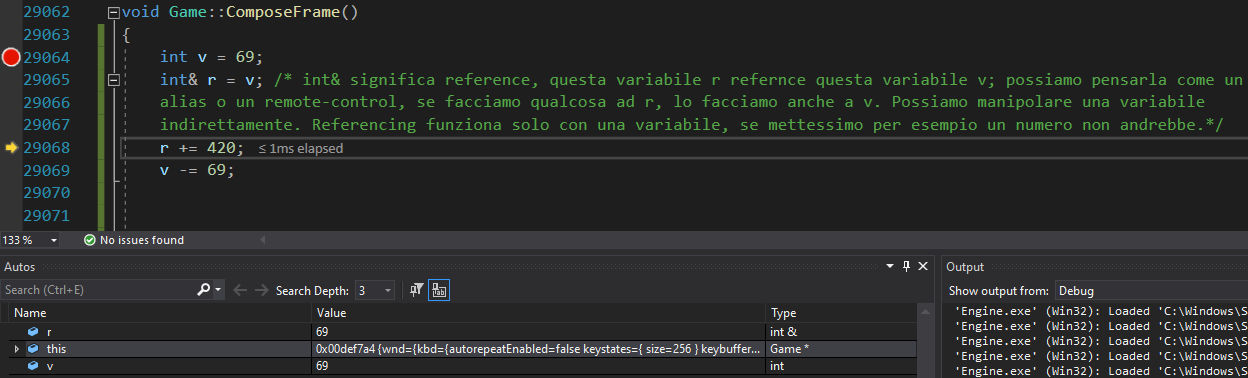
\includegraphics[width=1.2\textwidth, height=1.2\textheight, keepaspectratio]{./imgs/References.png}
	\caption{Reference}
	\label{fig:references1}
\end{figure}

\begin{figure}[ht]
	\centering
	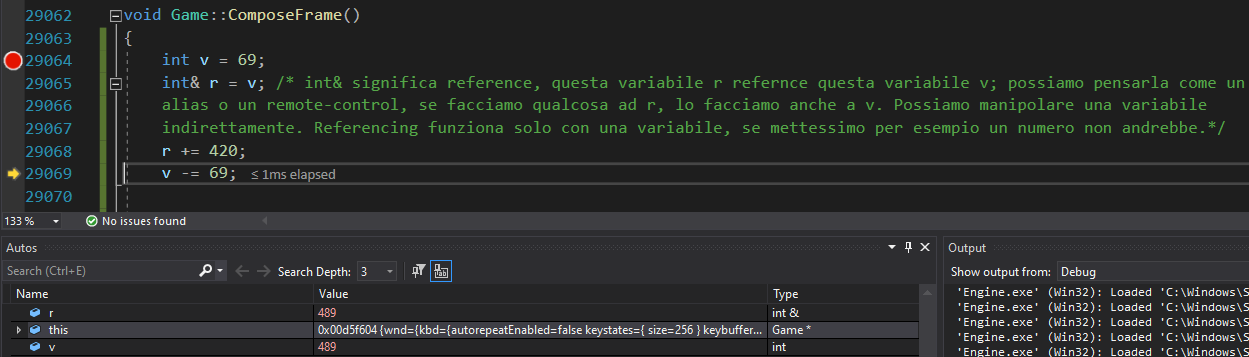
\includegraphics[width=1.2\textwidth, height=1.2\textheight, keepaspectratio]{./imgs/References2.png}
	\caption{Reference}
	\label{fig:references2}
\end{figure}

\subsection{References vs Puntatori}

\begin{tabular}{|c|c|}
	\hline
	\textbf{Reference} & \textbf{Pointers} \\
	\hline
	\textsf{\small Riferiscono ad una variabile } & \textsf{\small Memorizzano un indirizzo } \\
	\textsf{\small con un altro nome} & \textsf{\small di una variabile} \\
	\hline
	\textsf{\small Non possono avere un valore \color{myblue2}NULL \normalcolor.} & \textsf{\small Possono avere un valore \color{myblue2}NULL \normalcolor.} \\
	\hline
	\textsf{\small Deve essere inizializzata } & \textsf{\small Può anche non essere inizializzata } \\
	\textsf{\small alla dichiarazione} & \textsf{\small alla dichiarazione} \\
	\hline
	\textsf{\small Condivide la stessa memoria con la variabile originale, } & \textsf{\small Ha un proprio spazio e } \\
	\textsf{\small ma prende anche dello spazio nello stack.} & \textsf{\small indirizzo di memoria sullo stack.} \\
	\hline
	\textsf{\small Non può essere riassegnato.} & \textsf{\small Può essere riassegnato.} \\
	\hline
	\textsf{\small Hanno un solo livello di indirezione.} & \textsf{\small Si possono avere puntatori } \\
	\textsf{\small } & \textsf{\small a puntatori per livelli extra } \\
	\textsf{\small } & \textsf{\small di indirezione.} \\
	\hline
	\textsf{\small Non c'è la aritmetica delle references} & \textsf{\small C'è l'aritmetica dei puntatori.} \\
	\hline
	%\textsf{\small } & \textsf{\small } \\
	%\hline
\end{tabular}

% -------------------------- SECTION: STRINGHE ---------------------------------------

\newpage

\section{Stringhe}

%TODO: mettere std::string qui? E anche char? e c-strings? anche la Tabella ASCII?
%Prima questa parte dei char, C-string, std::string stava nella sezione Tipi di Dati

\subsection{Char}

\textsf{\small \textbf{Definizione: } Un \textbf{char} è usato per memorizzare un singolo carattere} \\

\textsf{\small Alternativamente, si possono usare i valori ASCII per indentificare le lettere} \\

\begin{lstlisting}
	char linguaggio = 'C';
	
	char linguaggio = 67; // 67 corrisponde a C nella tabella ASCII.
\end{lstlisting}

\subsection{C-string}

\textsf{\small Per creare una stringa in C facciamo un array (contenitore di dati dello stesso tipo) di char.}

\textsf{\small Il \textbf{'\textbackslash0'} è il \textbf{NUL terminator} che denota la fine di una C-stringa. } \\

\begin{lstlisting}
	char s[] = "prova";
	
	// Oppure possiamo scriverlo:
	char s[] = { 'p', 'r', 'o', 'v', 'a', '\0'};
	
	// '\textbackslash0' è il NUL terminator, denota la fine di una stringa.
\end{lstlisting}

\subsection{char*}

\textsf{\small Un puntatore a char memorizza la locazione iniziale di una C-string (una stringa in C). } \\

\begin{lstlisting}
	char s = "prova";
	
	// Possiamo far puntatore al puntatore la prima cella dell'array così..
	char* p = &(s[0]);
	
	// ..oppure in maniera più coincisa così:
	char *p = s;
\end{lstlisting}

\subsection{Tabella ASCII}

\textsf{\small \textbf{Definizione: } La tabella \textbf{ASCII} (\emph{American Standard Code for Information Interchange}) è un codice per la codifica di caratteri.} \\

\textsf{\small Inizialmente era basata su codici di 7 bit, quindi per un totale di $2^7 = 128$ caratteri. Venne poi estesa ad 8 bit, per un totale di $2^8 = 256$ caratteri.} \\

\begin{figure}[ht]
	\centering
	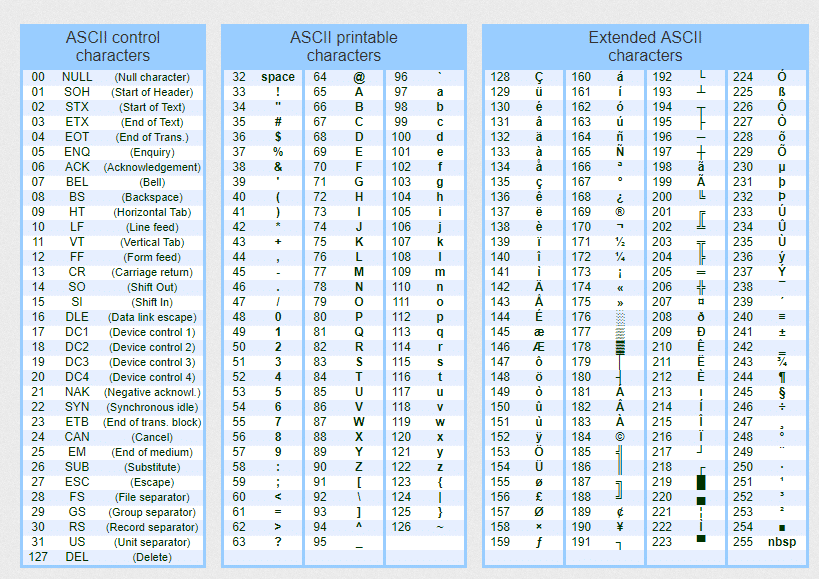
\includegraphics[width=1.2\textwidth, height=1.2\textheight, keepaspectratio]{./imgs/ascii_table2.png}
	\caption{Tabella ASCII}
	\label{fig:ascii_table}
\end{figure}

\subsection{std::string}

\textsf{\small \textbf{Definizione: } Il C++ ha una propria definizione per rappresentare una sequenza di caratteri come un oggetto di una classe. Questa classe è chiamata std::string. Questa memorizza i caratteri come una sequenza di bytes con la funzionalità di poter accedere al singolo carattere byte.} \\

\textsf{\small La classe std::string ha diverse funzioni, come: } 

\begin{tabular}{|c|c|}
	\hline
	\textbf{Funzione} & \textbf{Definizione} \\
	\hline
	\textbf{length()} & \textsf{\small restituisce la lunghezza della stringa.} \\
	\hline
	\textbf{capacity()} & \textsf{\small restituisce la capacità allocata alla stringa che } \\
	\textbf{} & \textsf{\small può essere più o meno la lunghezza.} \\
	\hline
	\textbf{resize()} & \textsf{\small cambia la grandezza della stringa che può essere aumentata o diminuita.} \\
	\hline
	\textbf{shrink\_to\_fit()} & \textsf{\small diminuisce la grandezza della stringa e la rende uguale } \\
	\textbf{} & \textsf{\small al minimo della capacità della stringa.} \\
	\textbf{} & \textsf{\small Utile per salvare ulteriore memoria se siamo sicuri } \\
	\textbf{} & \textsf{\small di non dover aggiungere altri caratteri.} \\
	\hline
	%\textbf{} & \textsf{\small } \\
\end{tabular} 

\textsf{\small Queste sono solo alcune delle funzioni della classe string.} \\

\begin{lstlisting}
	std::string str = "Ciao a tutti";
	
	str.resize(4); 
	
	std::cout << "Stringa dopo resize: " << str << std::endl; // Output : Stringa dopo resize: Ciao
	
	std::cout << "Capacità della stringa: " << str.capacity() << std::endl; // Output : Capacità della stringa: 12
	
	std::cout << "Lunghezza della stringa: " << str.length() << std::endl; // Output : Lunghezza della stringa: 4
	
\end{lstlisting}

\subsection{char* vs std::string vs char[]}

\subsubsection{Usare char*}

\begin{lstlisting}
	char *str = "prova";
\end{lstlisting}

\begin{tabular}{|c|c|}
	\hline
	\color{red} CONS & \color{Green} PROS \\
	\hline
	\textsf{\small In C va bene, ma in C++ è deprecato,  } & \textsf{\small Basta un singolo puntatore per  } \\
	\textsf{\small perché in C le stringhe sono array di char,} & \textsf{\small l'intera stringa. È efficiente } \\
	\textsf{\small mentre in C++ sono array di char costanti.} & \textsf{\small a livello di memoria.} \\
	\hline
	\textsf{\small Non possiamo modificare la stringa dopo, } & \textsf{\small Non c'è bisogno  } \\
	\textsf{\small possiamo semplicemente far puntare ad un'altra stringa.} & \textsf{\small di dichiarare la lunghezza } \\
	\textsf{\small } & \textsf{\small della stringa all' inizializzazione.} \\
	\hline
\end{tabular}

\subsubsection{Usare std::string}

\begin{lstlisting}
	std::string s = "prova";
\end{lstlisting}

\begin{tabular}{|c|c|}
	\hline
	\color{red} CONS & \color{Green} PROS \\
	\hline
	\textsf{\small } & \textsf{\small Con C++ std::string è la migliore via,  } \\
	\textsf{\small } & \textsf{\small perché ha delle funzioni di ricerca,} \\
	\textsf{\small } & \textsf{\small rimpiazzo e manipolazione migliori.} \\
	%\textsf{\small } & \textsf{\small } \\
	\hline
\end{tabular}

\subsubsection{Casi in cui preferire char* ad std::string}

\begin{itemize}
	\item \textsf{\small Quando si ha a che fare con livelli bassi di accesso, come interagire con il sitema operativo. Anche se std::string::c\_str dovrebbe occuparsi di quello.}
	\item \textsf{\small Compatibilità con del vecchio codice in C (Anche se la funzione std::string::c\_str dovrebbe già in largo modo occuparsi di questo).}
	\item \textsf{\small Per risparmiare memoria (std::string sicuramente occupa di più).}
\end{itemize}

\subsubsection{Usare char[]}

\begin{lstlisting}
	// In realtà ci bastano 5 spazi nell'array, però se poi dopo vogliamo fare
	// concatenazioni o manipolazioni sulle altre stringhe, ci servirà altro spazio.
	char stringa[128] = "prova";
\end{lstlisting}

\begin{tabular}{|c|c|}
	\hline
	\color{red} CONS & \color{Green} PROS \\
	\hline
	\textsf{\small È un array allocato staticamente che } & \textsf{\small Possiamo modificare la stringa } \\
	\textsf{\small consuma spazio nello stack.} & \textsf{\small anche in un altro stage del programma.} \\
	\hline
	\textsf{\small Dobbiamo utilizzare array di grandi dimensioni  } & \textsf{\small } \\
	\textsf{\small per poter concatenare o manipolare le altre stringhe,} & \textsf{\small } \\
	\textsf{\small visto che lo spazio dell'array è fissato dall'inizio.} & \textsf{\small } \\
	\hline
\end{tabular}

% -------------------------- SECTION: FUNZIONI ---------------------------------------

\newpage

\section{Funzioni}

\textsf{\small \textbf{Definizione: } Una funzione è un blocco di codice che esegue una specifico compito e può essere richiamato quando si vuole.} \\

\textsf{\small Le funzioni sono composte da: un tipo di dato di ritorno che è ciò che la funzione restituisce dopo esser stata eseguita, un nome, degli eventuali parametri ed racchiusa tra due parentesi graffe il corpo, il blocco di codice.}

\textsf{\small Per eseguire la funzione basta richiamarla col suo nome e passare gli eventuali parametri.} \\

\subsection{return}

\textsf{\small La keyword \textbf{return} permette di restituire un valore/oggetto dalla funzione.} \\

\begin{lstlisting}
	// tipologia nome\_funzione(parametri)
	{
		// Blocco di codice della funzione.
	}
	
	// Questa funzione restituisce un intero, si chiama somma, prende due parametri interi a e b e restituisce la somma tra a e b. 
	int somma(int a, int b){
		return a + b;
	}
	
	// Fuori dalla funzione
	int x = 3, y = 5;
	// chiamiamo la funzione somma, gli passiamo i parametri e il valore di ritorno lo assegniamo alla variabile intera z.
	int z = somma(x, y); // Output z : 8
\end{lstlisting}

\textsf{\small Tutto ciò che è creato all'interno della funzione è locale alla funzione e quindi non accessibile da fuori.} \\

\textsf{\small I nomi dei parametri sono soltanto dei placeholders. Potremmo anche non metterli e lasciare solo le tipologie, ma poi per poterli referenziare nella funzione non sapremmo come fare.}

\textsf{\small I parametri che vengono passati alla funzione sono anch'essi locali, a meno che non li si passano attraverso dei puntatori.} \\

\textsf{\small I parametri passati, a meno che con puntatori, sono delle copie delle variabili passate come parametro, e qualsiasi modifiche di queste copie non ha un effetto sui parametri passati.} \\

\begin{lstlisting}
	// Questa è una funzione che restituisce un boolean (0 o 1 (VERO o FALSO)), chiamata isGreater che prende due variabili intere a e b come parametri e restituisce se true se la variabile a è maggiore della variabile b, altrimenti false.
	
	// Questa funzione si potrebbe scrivere così..
	bool isGreater(int a, int b)
	{
		if(a > b){
			return a;
		} else {
			return b;
		}
	}

	//.. Oppure si potrebbe anche scrivere così.
	bool isGreater(int a, int b)
	{
		return a > b;
	}

	// Detto questo, per questo tipo di operazioni, ci sono già delle funzioni della libreria Standard ben più ottimizzate. Per questo esempio si potrebbe usare std::max.
\end{lstlisting}

\subsection{void}

\textsf{\small Se non volessimo ritornare niente dovremmo usare la tipologia \textbf{void}, questo tipo di funzione (che non ritorna niente) è chiamata \textbf{procedura}.} \\

\subsection{main}

\textsf{\small Il \textbf{main} è la funzione principale di qualsiasi programma in C/C++, da esso parte il tutto, ha origine tutto.} \\

\begin{lstlisting}
	int main(){
		return 0;
	}
\end{lstlisting}

\subsection{Funzioni ricorsive}

\textsf{\small Le funzioni ricorsive sono delle funzioni che richiamano se stesse per raggiungere un risultato.} \\

%TODO: fixare funzioni
\begin{lstlisting}
	// Il fattoriale di un numero, o anche scritto n! è n * (n - 1)
	// 4! = 4 * 3 * 2 * 1 = 24
	int fattoriale(int n)
	{
		if((n == 0) || (n == 1))
			return 1;
		else
			return n * fattoriale(n - 1);
	}

	// Questa funzione si potrebbe anche scrivere //TODO: Scherzavo non funziona
	int fattoriale(int n)
	{
		(n == 0) || (n == 1) ? return 1 : return n * fattoriale(n - 1);
	}

	// Fibonacci è una serie in cui i due primi elementi sono 1 e dove ogni elemento è uguale alla somma dei due termini precedenti. 
	
	//TODO: Scherzavo non funziona
	int fibonacci(int x)
	{
		((x == 1) || (x == 0)) ? return(x) : return(fibonacci(x - 1) + fibonacci(x - 2));
	}

	int main()
	{
		int x = 4;
		std::cout << "Fattoriale di " << x << " e\': " << fattoriale(x) << std::endl; // Output : Fattoriale di 4 è 24.
		
		int y = 15;
		std::cout << "Fibonacci di " << y << " e\' " << fibonacci(15) << std::endl; // Output : Fibonacci di 15 è 610.
		return 0;
	}
\end{lstlisting}

%TODO: funzioni e i vari casi dei const e dove viene posizionato.

%TODO: funzioni pass by value, by reference, ecc..

\subsection{Argomenti passati per valore}

\textsf{\small Quindi, quando passiamo dei valori (e non degli indirizzi di memoria alle variabili), si dice che passiamo gli argomenti \textbf{per valore}, quindi una copia delle variabili passate viene creata ed usata nelle funzioni. }

\textsf{\small Quindi noi non operiamo direttamente sulle variabili passate, ma sulle loro copie. Questo non ci permette di poter modificare le variabili passate.} \\

\begin{lstlisting}
	int sottrazione(int a, int b)
	{
		return a - b;
	}

	// Fuori dalla funzione
	int x = 5, y = 3;
	int z = sottrazione(x, y); // Output: 2
\end{lstlisting}

\subsection{Argomenti passati per referenza}

\textsf{\small Per poter effettivamente modificare le variabili che abbiamo passato per argomento, dobbiamo passarle con i puntatori, dobbiamo passare i loro indirizzi di memoria. Questo si chiama passare argomenti \textbf{per referenza}.} \\

\textsf{\small Se, per esempio, volessimo sostituire i valori di due variabili e li passassimo per valore, non riusciremmo.} \\

\begin{lstlisting}
	// Parte 1: Usare argomenti passati per valore.
	void swap(int a, int b)
	{
		int temp = a;
		a = b;
		b = temp;
	}

	// Fuori dalla funzione
	int x = 5, y = 3;
	swap(x, y); 
	std::cout << "Valore di x dopo lo swap: " << x << std::endl; // Output : 5
	std::cout << "Valore di y dopo lo swap: " << y << std::endl; // Output : 3
	// Non funziona, noi vorremmo cambiare i valori di x ed y, ma così non funziona, perchè stiamo lavorando sulle copie delle variabili, non sulle variabili stesse.
	
	// Parte 2: Usare argomneti passati per referenza
	void swap(int *a, int *b)
	{
		int temp = *a;
		*a = *b;
		*b = temp;
	}

	// Fuori dalla funzione
	int x = 5, y = 3;
	swap(x, y);
	std::cout << "Valore di x dopo lo swap: " << x << std::endl; // Output : 3
	std::cout << "Valore di y dopo lo swap: " << y << std::endl; // Output : 5
	
	// Ha funzionato, perché abbiamo agito sulle variabili passate e non sulle loro copie.
	
	// Quello visto prima ero un modo per poter fare la funzione swap in C che funziona anche in C++, ma c'è anche un altro modo ovvero utilizzando le references.
	
	void swap(int &a, int &b)
	{
		int temp = a;
		a = b;
		b = temp;
	}

	// Fuori dalla funzione
	int x = 5, y = 3;
	swap(x, y);
	std::cout << "Valore di x dopo lo swap: " << x << std::endl; // Output : 3
	std::cout << "Valore di y dopo lo swap: " << y << std::endl; // Output : 5
	
	// Comunque c'è una funzione della libreria Standard std::swap() per questo.
\end{lstlisting}

\subsection{Funzioni che ritornano puntatori}

\textsf{\small Si possono, naturalmente, ritornare i puntatori dalle funzioni.}

\begin{lstlisting}
	int* func()
	{
		static int a = 11; // static così rimane sempre in memoria anche quando non si chiama la funzione
		return &a;
	}

	int *p;
	
	p = func();
	
	std::cout << p << std::endl; // Output : indirizzo di p
	std::cout << *p << std::endl; // Output : 11
\end{lstlisting}

%TODO: magari scrivere a cosa possa essere utile ritornare i puntatori dalle funzioni.
%TODO: Puntatori a funzioni nel capitolo advanced.

% -------------------------- SECTION: VARIABLES SCOPE --------------------------------

\section{Variables Scope}

\textsf{\small Variables Scopes, o in italiano, la portata delle variabili, significa fino a dove una variabile può essere utilizzata, fino a dove esiste, vale, la possiamo usare.} \\

\textsf{\small La portata è una regione del programma, ci sono all'incirca 3 principali posti in cui le variabili possono essere dichiarate ed in base a questo le variabili assumono diversi nomi: }

\begin{itemize}
	\item \textsf{\small \textbf{Locali} : dentro ad una funzione o ad un blocco di codice (racchiuso tra le graffe).}
	\item \textsf{\small \textbf{Parametri formali} : ovvero nella definizione della funzione, nei suoi parametri.}
	\item \textsf{\small \textbf{Globale} : fuori dalle funzioni.}
\end{itemize}

\subsection{Variabili Locali}

\textsf{\small Le variabili create all'interno di una funzione o un blocco di codice, sono locali a quella funzione, possono essere utilizzate solo all'interno di quella funzione e non all'esterno. Una volta che la funzione termina, quella variabile cessa di esistere.} \\

\begin{lstlisting}
	void funzione()
	{
		int a = 5;
		std::cout << "Valore variabile locale a: " << a << std::endl;
	}
	
	// Fuori dalla funzione
	funzione(); // Output : Valore variabile locale a: 5
	
	std::cout << "Valore variabile locale a: " << a << std::endl; // Errore la variabile a non esiste!
\end{lstlisting}

\subsection{Parametri formali}

\textsf{\small Sono i parametri della funzione, esistono soltanto finchè la funzione esiste.} \\

\begin{lstlisting}
	void funzione(int a)
	{
		std::cout << "Valore variabile a: " << a << std::endl;
	}
	
	int main()
	{
		int x = 8;
		funzione(x); // Output Valore variabile a: 8
		
		std::cout << "Valore variabile a: " << a << std::endl; // Errore non esiste in questo scope.
		
		return 0;
	}
\end{lstlisting}

\subsection{Variabili Globali}

\textsf{\small Esistono per tutta la durata del programma, posso essere utilizzate anche all'interno delle funzioni e il loro valore non viene perso una volta che la funzione smette.} \\

\begin{lstlisting}
	int x = 10;
	
	void funzione()
	{
		std::cout << "Valore variabile x: " << x << std::endl;
	}
	
	int main()
	{
		funzione(); // Output Valore variabile x: 10
		return 0;
	}
\end{lstlisting}

% -------------------------- SECTION: HEADERS ----------------------------------------

\newpage

\section{Header files}

\textsf{\small \textbf{Definizione: } Gli header files, o file di intestazione in italiano, sono dei files con l'estensione \textbf{.h} o \textbf{.hpp} che contengono le dichiarazioni delle funzioni e definizione di macro e tipi.}\\

\textsf{\small Sono un modo per organizzare il codice, possiamo includere gli elementi di questi files nel nostro codice attraverso la direttiva \textbf{\#include} che informa il preprocessore di cercare questo file prima di continuare ad eseguire il codice. } 

\textsf{\small Esistono due tipi di header files: quelli standard del linguaggio/compilatore e quelli creati dall'utente programmatore.}

\textsf{\small Per includere le librerie standard usiamo \textbf{\#include <nomelibreria>} perché il compilatore sa dove si trovano queste librerie, mentre per le librerie definite dall'utente usiamo \textbf{\#include "nomelibreria.h"} e passiamo anche il percorso di dove si trova. (ammeno che non si trova nella stessa cartella in cui si trova il nostro codice, in quel caso basta mettere il nome della libreria)} \\

% \texorpdfstring % per inserire caratteri speciali nelle section, subsection, ecc..
\subsection{Only Once Headers | pragma once | ifndef}

\textsf{\small \textbf{Definizione: } Se un file header viene incluso due volte, il compilatore lo processerà il suo contenuto due volte, il che risulterà in un errore. Per evitare questo c'è una procedura standard da scrivere all'interno del file di intestazione.}

\begin{lstlisting}
	#ifndef NOME_HEADER_FILE_H
	#define NOME_HEADER_FILE_H
	
	// Tra queste c'è il codice dell'header file.
	
	#endif
\end{lstlisting}

\textsf{\small La direttiva \textbf{\#ifndef} controlla che il file non sia già stato aggiunto, se non è mai stato aggiunto, allora lo aggiunge, altrimenti salta il contenuto così che non verrà aggiunto due volte.} \\

\textsf{\small Inoltre, per fare questa stessa operazione, ma più semplice e corta esiste una direttiva non-standard: \textbf{\#pragma once}. } 

\begin{lstlisting}
	#pragma once
	
	// Contenuto dell'header.
\end{lstlisting}

\subsection{Cosa sono le librerie?}

\textsf{\small Le librerie sono collezioni di risorse non volatili usate dai programmi. La libreria Standard è una collezione di classi, funzioni, macros, costanti, ecc.. che sono state scritte in C++ stesso. Ci sono una grande lista di header files che contengono i contenuti della libreria Standard.} \\

\subsection{Header files libreria Standard}

\textsf{\small Qui, una lista degli header files della libreria standard più comuni (alcuni anche del C): } \break

\begin{comment}
\begin{itemize}
	\item \textsf{\small \textbf{\#include <stdio.h>} : per l'input ed output (dal C).}
	\item \textsf{\small \textbf{\#include <iostream>} : input ed output fondamentali.}
	\item \textsf{\small \textbf{\#include <string>} : fornisce le standard classi string e template.}
	\item \textsf{\small \textbf{\#include <math.h>} : per operazioni matematiche (dal C).}
	\item \textsf{\small \textbf{\#include <limits>} : usata per descrivere proprietà di tipi numerici fondamentali.}
	\item \textsf{\small \textbf{\#include <time.h>} : per funzioni legate al tempo (dal C).}
	\item \textsf{\small \textbf{\#include <chrono>} : fornisce elementi di tempo, come std::chrono::duration e std::chrono::time\_point ed altri.}
	\item \textsf{\small \textbf{\#include <algorithm>} : fornisce la definzione di molti container algoritmici.}
	\item \textsf{\small \textbf{\#include <iterator>} : fornisce templates e classi per lavorare con gli iteratori.}
	\item \textsf{\small \textbf{\#include <sstream>} : fornisce delle classi per la manipolazione di stringhe.}
	\item \textsf{\small \textbf{\#include <vector>} : fornisce la classe di template container std::vector, un array dinamico.}
	\item \textsf{\small \textbf{\#include <random>} : facilita la generazione di numeri (pseudo-)casuali e distribuzioni.}
	\item \textsf{\small \textbf{\#include <numeric>} : operazioni numeriche generalizzate.}
	\item \textsf{\small \textbf{\#include <functional>} : fornisce diverse oggetti funzionali da usare con gli standard algorithm.}
	\item \textsf{\small \textbf{\#include <stdexcept>} : classi per le eccezioni.}
	\item \textsf{\small \textbf{\#include <memory>} : per la gestione della memoria.}
	\item \textsf{\small \textbf{\#include <optional>} : per gli opzionali.}
	\item \textsf{\small \textbf{\#include <ranges>} : per i ranges e per i lazy evaluated adaptors. (C++20)}
	\item \textsf{\small \textbf{\#include <concepts>} : fornisce la libreria fondamentale concepts. (C++20)}
	\item \textsf{\small \textbf{\#include <thread>} : fornisce classi e namespaces per lavorare sui threads.}
	%\item \textsf{\small \textbf{\#include <>} : }
\end{itemize}
\end{comment}

\begin{tabular}{cc}
	\textbf{\#include <stdio.h>} : & \textsf{\small per l'input ed output (dal C).} \\
	\textbf{\#include <iostream>} : & \textsf{\small input ed output fondamentali.} \\
	\textbf{\#include <string>} : & \textsf{\small fornisce le standard classi string e template.} \\
	\textbf{\#include <math.h>} : & \textsf{\small per operazioni matematiche (dal C).} \\
	\textbf{\#include <limits>} : & \textsf{\small usata per descrivere proprietà di tipi numerici fondamentali.} \\
	\textbf{\#include <time.h>} : & \textsf{\small per funzioni legate al tempo (dal C).} \\
	\textbf{\#include <chrono>} : & \textsf{\small fornisce elementi di tempo, come std::chrono::duration e } \\
	\textbf{} & \textsf{\small std::chrono::time\_point ed altri.} \\
	\textbf{\#include <algorithm>} : & \textsf{\small fornisce la definzione di molti container algoritmici.} \\
	\textbf{\#include <iterator>} : & \textsf{\small fornisce templates e classi per lavorare con gli iteratori.} \\
	\textbf{\#include <sstream>} : & \textsf{\small fornisce delle classi per la manipolazione di stringhe.} \\
	\textbf{\#include <vector>} : & \textsf{\small fornisce la classe di template container std::vector, } \\
	\textbf{} & \textsf{\small un array dinamico.} \\
	\textbf{\#include <random>} : & \textsf{\small facilita la generazione di numeri (pseudo-)casuali } \\
	\textbf{} & \textsf{\small e distribuzioni.} \\
	\textbf{\#include <numeric>} : & \textsf{\small operazioni numeriche generalizzate.} \\
	\textbf{\#include <functional>} : & \textsf{\small fornisce diverse oggetti funzionali da usare } \\
	\textbf{} & \textsf{\small con gli standard algorithm.} \\
	\textbf{\#include <stdexcept>} : & \textsf{\small classi per le eccezioni.} \\
	\textbf{\#include <memory>} : & \textsf{\small per la gestione della memoria.} \\
	\textbf{\#include <optional>} : & \textsf{\small per gli opzionali.} \\
	\textbf{\#include <ranges>} : & \textsf{\small per i ranges e per i lazy evaluated adaptors. (C++20)} \\
	\textbf{\#include <concepts>} : & \textsf{\small fornisce la libreria fondamentale concepts. (C++20)} \\
	\textbf{\#include <thread>} : & \textsf{\small fornisce classi e namespaces per lavorare sui threads.} \\
\end{tabular} \break

\textsf{\small Inoltre, tutti gli headers dalla libreria standard del C sono inclusi nella libreria standard del C++}

\textsf{\small Ci sono tanti altri headers file e ognuno usato per qualcosa..} \\

\subsection{Librerie create dagli utenti}

\textsf{\small Gli utenti si possono creare le proprie librerie, creando un file \textbf{.h} con le sole definizioni di funzioni e un file chiamato come l'header file, con le implementazioni di queste, ma con l'estensione \textbf{.cpp}.}

\textsf{\small Per includere queste librerie, usiamo \textbf{\#include "nome\_libreria.h"}, al posto di \textbf{\#include <nomelibreria.h>}, perché non una libreria standard e quindi il compilatore non sa dove cercarla e quindi gli dobbiamo specificare noi dove si trova la nostra libreria.} \\

\begin{lstlisting}
	// Nel file header nomelibreria.h
	int somma(int a, int b);
	
	// Nel file .cpp nomelibreria.cpp
	#include "nomelibreria.h"
	
	int somma(int a, int b){
		return a + b;
	}
\end{lstlisting}

\subsection{Differenza tra .h vs .hpp}

\textsf{\small In C++ l'estensione del file non è importante. L'uso di .h , .hpp, .hxx, .hh, .tpp o nessuna estensione sono tutte convenzioni.} \\

\begin{tabular}{|c|c|}
	\hline
	\textbf{.h} & \textbf{.hpp} \\
	\hline
	\textsf{\small Sia per il C che per il C++} & \textsf{\small È solo per C++} \\
	\textsf{\small Dal punto di vista del C++, } & \textsf{\small Non funzionerà con il C.} \\
	\textsf{\small il codice C verrà definito come \emph{extern "C"}} & \textsf{\small } \\
	\textsf{\small Esprime l'intento che si usa il C } & \textsf{\small Esprime l'intento che si usi C++} \\
	\textsf{\small (o perlomeno si può pensare così)} & \textsf{\small (o perlomeno si può pensare così)} \\
	\textsf{\small Dal punto di vista del C, il codice C sarà visibile, } & \textsf{\small } \\
	\textsf{\small mentre quello del C++ sarà invisibile.} & \textsf{\small } \\
	\hline
\end{tabular}

%TODO: cosa sono le librerie? Questi sono solo file di intestazioni.

% -------------------------- SECTION: NAMESPACES -------------------------------------

\newpage

\section{Namespaces}

\textsf{\small \textbf{Definizione: } Gli \textbf{namespaces} ci permettono di raggruppare varie entità che altrimenti si troverebbero nello scope globale. Permettono una migliore organizzazione e strutturazione del codice.} \\

\textsf{\small Se avessimo per esempio due funzioni con lo stesso nome, sarebbe difficile differenziarle e quindi i namespaces ci permettono di separarle.}

\textsf{\small Per creare una namespace adoperiamo la keyword \textbf{namespace}.} \\

\begin{lstlisting}
	namespace primo_spazio {
		void func()
		{
			std::cout << "Dentro al namespace: primo_spazio" << std::endl;
		}
	}

	namespace secondo_spazio {
		void func()
		{
			std::cout << "Dentro al namespace: secondo_spazio" << std::endl;
		}
	}

	int main()
	{
		// Chiamo la funzione func del primo spazio.
		primo_spazio::func();
		// Output: Dentro al namespace: primo\_spazio
		
		// Chiamo la funzione func del secondo spazio.
		secondo_spazio::func();
		// Output: Dentro al namespace: secondo\_spazio
		return 0;
	}
\end{lstlisting}

\textsf{\small Il namespace più usato è quello della libreria Standard del linguaggio, ovvero il namespace std che raggruppa tutte le funzioni e classi della libreria Standard. } \\

\textsf{\small Ogni qualvolta che usiamo una funzione, classe della libreria Standard ci riferiamo a quel namespace. Usiamo il nome del namespace e i due punti :: per indicare che quello che stiamo usando fa parte di quel namespace. C'è un modo, però per evitare ogni volta di scrivere std::, ed è attraverso la riga \textbf{using namespace std;}. Con questo non abbiamo più bisogno di scrivere std::, perché lo da già per scontato, o meglio, li prende direttamente dalla libreria Standard.} \\

\begin{lstlisting}
	// Accediamo al namespace std.
	std::string s = "Hello World!";
	
	// Qui invece facciamo la stessa cosa, ma senza dover riscrivere ogni volta std::
	using namespace std;
	
	string s = "Hello World!";
\end{lstlisting}


\subsection{std:: vs using namespace std}

\textsf{\small Usare \textbf{using namespace std} è considerato una \textbf{\color{red}bad practice}, probabilmente ci sono diversi motivi per questo, ma qui ne elenco alcuni: } \\

\begin{itemize}
	\item \textsf{\small Come abbiamo detto prima, se noi per esempio abbiamo due namespaces con due funzioni con lo stesso nome, se noi usiamo \emph{using namespace nome\_del\_namespace} allora avremmo un conflitto, o meglio, avremmo due namespaces con una funzione con lo stesso nome, il che creerebbe confusione. (e questo non vale solo per le funzioni, ma anche per le classi, costanti, ecc..). Il programma ancora compilerebbe, ma potrebbe chiamare la funzione sbagliata.}
	\item \textsf{\small Usare \emph{using namespace std} importerebbe nel nostro programma l'intero namespace std anche quando a noi serve solo una parte del namespace. \textbf{Non} è un problema di performance, ma solo di chiarezza del codice e di evitare ambiguità.}
	\item \textsf{\small Scrivere invece \textbf{std::} ogni volta rende chiaro il codice, perchè si capisce subito da quale namespace stai prendendo quella data funzione e/o altro.}
	%\item \textsf{\small }
\end{itemize}

\textsf{\small Quindi, per rendere il codice più chiaro è meglio usare \textbf{std::} al posto del using namespace std;} \\

\begin{lstlisting}
	// Se rimostrassimo il codice di prima
	
	namespace primo_spazio {
		void func()
		{
			std::cout << "Dentro al namespace: primo_spazio" << std::endl;
		}
	}
	
	namespace secondo_spazio {
		void func()
		{
			std::cout << "Dentro al namespace: secondo_spazio" << std::endl;
		}
	}

	using namespace primo_spazio;
	using namespace secondo_spazio;
	
	int main()
	{
		// Il codice diventa ambiguo!
		func();
		func();
		return 0;
	}
\end{lstlisting}

\textsf{\small Un modo per evitare questa ambiguità sarebbe usando la keyword \textbf{typedef} che permette essenzialmente di rinominare una keyword.}

\begin{lstlisting}
	// Questo eviterebbe in parte l'ambiguità, ma comunque rimane meglio mettere nome\_del\_namespace::funzione.
	typedef primo_spazio::func() primo_func();
	typedef secondo_spazio::func() secondo_func();
	
	int main()
	{
		// Chiamo la funzione func del primo spazio.
		primo_func();
		// Output: Dentro al namespace: primo\_spazio
		
		// Chiamo la funzione func del secondo spazio.
		secondo_func();
		// Output: Dentro al namespace: secondo\_spazio
		return 0;
	}
\end{lstlisting}

\textsf{\small Al posto di importare l'intero namespace std, si potrebbe troncare e portare solo una parte del namespace std.} \\

\begin{lstlisting}
	using std::cout;
	
	std::string s = "Hello World!"
	
	cout << s << std::endl;
\end{lstlisting}

\textsf{\small Comunque, in generale è meglio usare \textbf{std::}.} \\

\subsection{Mai mettere using namespace in un header file!}

\textsf{\small Un altro importante problema che può capitare con \textbf{using namespace std} è quello di includerlo in un header file. È DA \textbf{NON} FARE!} \\

\textsf{\small Mettere lo \textbf{using namespace} in un header file costringe chiunque voglia utilizzare la tua libreria ad usare anche \textbf{using namespace}, il che crea un problema quando per esempio l'utente crea una funzione che si trova anche nel namespace.}

\begin{figure}[ht]
	\centering
	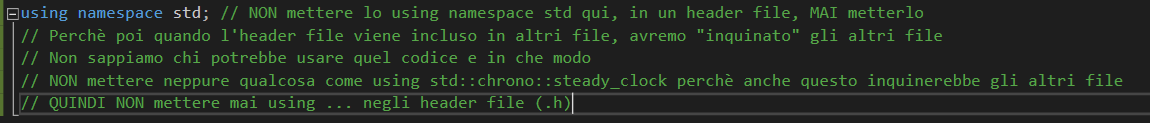
\includegraphics[width=1.2\textwidth, height=1.2\textheight, keepaspectratio]{./imgs/MAI_mettere_USING_negli_header_files.png}
	\caption{Mai mettere using in un header file}
	\label{fig:never_using_in_header}
\end{figure}

\textsf{\small Quindi, meglio mettere \textbf{using namespace} nei files \textbf{.cpp}, ma in generale, come abbiamo detto prima è meglio \textbf{non} utilizzarli.} \\

\textsf{\small Quindi \textbf{non} mettere \textbf{using namespace} in un header file, neanche \textbf{using namespace std}.} \\

% -------------------------- SECTION: STRUTTURE --------------------------------------

\newpage

\section{Strutture}

\textsf{\small \textbf{Definizione: } Le strutture sono dei tipi di dati definiti dall'utente per raggruppare oggetti di tipi diversi.} 

\textsf{\small Sono usati per rappresentare un record.}

\textsf{\small La keyword \textbf{struct} è usata per creare una struttura.}

\textsf{\small In questo modo semplicemente creiamo la struttura, ma non instanziamo nessun oggetto, per creare una istanza servirà richiamare il nome della struttura e poi il nome dell'istanza.}

\textsf{\small Per accedere ai campi della struttura si potrà usare l'operatore \textbf{.} (punto).}

\begin{lstlisting}
	struct nome_struttura{
		// campi della struttura
		int x;
		double d;
		char stringa[128];
	}; // Da notare il ; alla fine

	// Esempio una struttura per immagazzinare le coordinate di un punto.
	struct Point {
		int x;
		int y;
	};

	// In realtà in C++ non è necessario usare la keyword struct per creare un'istanza, a differenza del C.
	struct Point p1;
	p1.x = 0;
	p1.y = 1;
\end{lstlisting}

\textsf{\small In realtà in C++ non è necessario usare la keyword struct per creare un'istanza, a differenza del C.}

\textsf{\small Inoltre è anche possibile assegnare dei valori di default ai campi della struttura.} \\

\begin{lstlisting}
	struct Point{
		int x = 0;
		int y = 1;
	};

	struct Point p1;
	std::cout << p1.x << std::endl; // Output : 0
	std::cout << p1.y << std::endl; // Output : 1
\end{lstlisting}

\subsection{typedef}

\textsf{\small \textbf{Definizione: } La keyword \textbf{typedef} è usata essenzialmente per rinominare una tipologia.}

\textsf{\small Possiamo usare la parola chiave \textbf{typedef} per evitare di scrivere ogni volta struct nome\_della\_struttura per instanziare:} \\

\begin{lstlisting}
	typedef struct Point Punto;
	// Ora possiamo semplicemente scrivere Punto nome\_della\_istanza per creare una nuova istanza, al posto di dover scrivere struct Point nome\_della\_istanza.
	// In questo caso, potrebbe non sembrare molto, ma per strutture con nomi più lunghi è una manna dal cielo.
	
	Punto p1;
	p1.x = 3;
	p1.y = 2;
\end{lstlisting}

\textsf{\small Inoltre, ci sono diversi modi per creare una struttura apparte il modo visto prima, due di questi è attraverso il \textbf{typedef}: } \\

\begin{lstlisting}
	// Altro modo 1
	typedef struct Point {
		int x;
		int y;
	} Point;

	Point p1;
	p1.x = 1;
	p1.y = 0;
	
	// Altro modo 2
	struct Point {
		int x;
		int y;
	} typedef Point;

	Point p1;
	p1.x = 4;
	p1.y = 5;
\end{lstlisting}

\subsection{Funzioni nelle strutture} %TODO: oppure come subsection delle differenze C e C++

\textsf{\small A differenza del C, nelle strutture del C++ è possibile inserire delle funzioni.} \\

\begin{lstlisting}
	struct Rettangolo{
		int x;
		int y;
		int area(){
			return x * y;
		}
	};

	int main()
	{
		typedef struct Rettangolo Rettangolo;
		Rettangolo r1;
		r1.x = 3;
		r1.y = 2;
		std::cout << "Area rettangolo: " << r1.area() << std::endl; // Output : Area rettangolo: 6
		return 0;
	}
\end{lstlisting}

\subsection{Strutture nelle strutture}

\textsf{\small È possibile includere delle strutture all'interno di una struttura, come una matriosca.} \\

\begin{lstlisting}
	struct Point {
		int x;
		int y;
	};

	// Ovviamente la definizione della struttura Point deve essere fatta prima della struttura Rettangolo se la vogliamo includere in Rettangolo.
	struct Rettangolo{
		Point p;
		int area(){
			return p.x * p.y;
		}
	};

	typedef struct Rettangolo Rettangolo;
	Rettangolo r1;
	r1.p.x = 3;
	r1.p.y = 2;
	std::cout << "Area rettangolo: " << r1.area() << std::endl; // Output : Area rettangolo: 6
\end{lstlisting}

\subsection{Puntatore ad una struttura}

\textsf{\small È possibile far puntare un puntatore ad una struttura.} \\

\textsf{\small Per assegnare un valore ad uno specifico campo della struttura possiamo sia avvalerci dell'operatore \textbf{.} sia dell'operatore \textbf{->} che in questo caso fa esattamente la stessa cosa.} \\

\begin{lstlisting}
	struct Book {
		char  title[50];
		char  author[50];
		char  subject[100];
		int   book_id;
	};

	typedef struct Book Book;
	Book *pBook;
	
	// Possiamo sia fare così..
	(*pBook).title = "Learn C++";
	
	//.. sia fare così
	pBook->title = "Learn C++";
\end{lstlisting}

\subsection{Array di Strutture}

\textsf{\small Ovviamente è possibile creare un array di strutture, dove ogni elemento dell'array è una struttura.} \\

\begin{lstlisting}
	struct Cliente{
		int id;
		char nome[128];
	};

	typedef struct Cliente Cliente;
	
	Cliente clienti[2] = {{0, "Gigi"}, {1, "Pippo"}};
	// Oppure
	clienti[0].id = 0;
	clienti[0].nome = "Gigi";
	
	clienti[1].id = 1;
	clienti[1].nome = "Pippo";
	
	// Oppure si potrebbe anche fare così
	struct Cliente{
		int id;
		char nome[128];
	}cliente1, cliente2;

	cliente1.id = 0;
	cliente1.nome = "Gigi";
	
	cliente2.id = 1;
	cliente2.nome = "Pippo";
	
\end{lstlisting}

\subsection{Strutture come parametri e come ritorno}

\textsf{\small Ovviamente, si possono passare anche le strutture come parametri. Da fare attenzione che se non serve, meglio non copiare un'intera struttura quando la si passa come parametro.}

\begin{lstlisting}
	struct Book {
		char  title[50];
		char  author[50];
		char  subject[100];
		int   book_id;
	};
	
	void stampaLibro(struct Book* book){
		std::cout << "Titolo: " << book->title << std::endl;
		std::cout << "Autore: " << book->author << std::endl;
		std::cout << "Soggetto: " << book->subject << std::endl;
		std::cout << "Id: " << book->book_id << std::endl;
	}

	struct Book book1;
	std::strcpy( book1.title, "Learn C++ Programming");
	std::strcpy( book1.author, "Chand Miyan"); 
	std::strcpy( book1.subject, "C++ Programming");
	book1.book_id = 3;
	
	stampa(&book1);
	// Output : Titolo: Learn C++ Programming
	// Output : Autore: Chand Miyan
	// Output : Soggetto: C++ Programming
	// Output : Id: 3
\end{lstlisting}

\textsf{\small Al tempo stesso, si possono restituire strutture dalle funzioni.} \\

\begin{lstlisting}
	#define MATERIE 3
	
	struct studente{
		int matricola;
		char nome[128];
		char cognome[128];
		int voti[MATERIE];
		int media;
	};

	typedef struct studente Studente;
	
	// std::cin serve per l'input dell'utente.

	Studente createStudente(){
		Studente s;
		std:: cout << "Inserisci matricola: \n";
		std::cin >> s.matricola;
		
		std:: cout << "Inserisci nome: \n";
		std::cin >> s.nome;
		
		std:: cout << "Inserisci cognome: \n";
		std::cin >> s.cognome;
		
		int sum = 0;
		
		for(int i = 0; i < MATERIE; i++){
			std:: cout << "Inserisci voto: \n";
			std::cin >> s.voti[i];
			sum += s.voti[i];
		}
	
		s.media = sum / MATERIE;
		
		return s;
	}

	int main()
	{
		Studente s = createStudente();
		// Output : quelli inseriti
		std::cout << "Nome: " << s.nome << std::endl;
		std::cout << "Cognome: " << s.cognome << std::endl;
		std::cout << "Voto1: " << s.voti[0] << std::endl;
		std::cout << "Voto2: " << s.voti[1] << std::endl;
		std::cout << "Voto3: " << s.voti[2] << std::endl;
		std::cout << "Media: " << s.media << std::endl;
		return 0;
	}
\end{lstlisting}

\subsection{Strutture in C vs in C++}

\begin{tabular}{|c|c|}
	\hline
	\textbf{Strutture in C} & \textbf{Strutture in C++} \\
	\hline
	\textsf{\small Sono permessi solo membri dati, non funzioni.} & \textsf{\small Sono permessi sia dati sia funzioni membri.} \\
	\hline
	\textsf{\small Non può avere membri statici.} & \textsf{\small Può avere membri statici.} \\
	\hline
	\textsf{\small Non possiamo avere un costruttore.} & \textsf{\small Possiamo avere un costruttore.} \\
	\hline
	\textsf{\small L'inizializzazione diretta dei membri non è possibile.} & \textsf{\small L'inizializzazione diretta dei membri è possibile.} \\
	\hline
	\textsf{\small È necessario usare la keyword struct } & \textsf{\small Non è necessario usare la keyword struct.} \\
	\textsf{\small per dichiarare una variabile di tipo struct.} & \textsf{\small } \\
	\hline
	\textsf{\small Non supporta access modifiers.} & \textsf{\small Supporta gli access modifiers. } \\
	\textsf{\small } & \textsf{\small (public, private, protected, ecc..)} \\
	\hline
	\textsf{\small Sono permessi soltanto i puntatori alle strutture.} & \textsf{\small Sono permessi sia i puntatori sia le references.} \\
	\hline
	\textsf{\small L'operatore sizeof() genererà 0 } & \textsf{\small L'operatore sizeof() genererà 1 } \\
	\textsf{\small per una struttura vuota.} & \textsf{\small per una struttura vuota.} \\
	\hline
	\textsf{\small Il Data Hiding non è possibile.} & \textsf{\small Il Data Hiding è possibile.} \\
	\hline
\end{tabular}

% -------------------------- SECTION: UNION ------------------------------------------

\section{Union}

\textsf{\small \textbf{Definizione: } La \textbf{union} è un tipo di struttura dove l'ammontare di memoria è una fattore chiave.} \\

\begin{itemize}
	\item \textsf{\small Come le strutture, le union possono contenere diversi tipologie di variabili.}
	\item \textsf{\small Ogni qualvolta che una nuova variabile è inizializzata dall'union in C sovrascrive quella vecchia, ma in C++ usiamo quella locazione di memoria e non abbiamo bisogno di quella parola chiave.}
	\item \textsf{\small È utile quando i dati passati ad una funzione sono sconosciuti, utilizzare una \textbf{union} che contiene tutti i possibili tipi può essere il rimedio a questo problema.}
	\item \textsf{\small Utilizziamo la keyword \textbf{union} per crearne una.}
\end{itemize}

\begin{lstlisting}
	union nome_della_union {
		// tipi di dati
	}; // Da notare il ; proprio come nelle strutture.

	union var {
		int iVar;
		char cVar;
		float fVar;
	};

	int main()
	{
		// In C++ non serve la keyword union.
		union var V1, V2, V3;
		
		V1.iVar = 33;
		V2.cVar = 33;
		V3.fVar = 33.33;
		
		std::cout << "V1 var: " << V1.iVar << std::endl; // Output : V1 var: 33
		std::cout << "V2 var: " << V2.cVar << std::endl; // Output : V2 var: !
		std::cout << "V3 var: " << V3.fVar << std::endl; // Output : V3 var: 33.33
		
		return 0;
	}
\end{lstlisting}

\subsection{structure vs union}

\begin{tabular}{|c|c|}
	\hline
	\textbf{Structure} & \textbf{Union} \\
	\hline
	\textsf{\small Usa la keyword \textbf{struct}} & \textsf{\small Usa la keyword \textbf{union}}\\
	\hline
	\textsf{\small Quando una variabile è associata con una struttura} & \textsf{\small Quando una variabile è associata con } \\
	\textsf{\small il compilatore alloca la memoria } & \textsf{\small una union il compilatore alloca memoria } \\
	\textsf{\small per ogni membro.} & \textsf{\small considerando lo spazio occupato } \\
	\textsf{\small Lo spazio occupato dalla struttura} & \textsf{\small dal membro più grande.} \\
	\textsf{\small è maggiore o uguale alla somma} & \textsf{\small } \\
	\textsf{\small dello spazio dei suoi membri.} & \textsf{\small } \\
	\hline
	\textsf{\small Per ogni membro della struttura} & \textsf{\small La memoria allocata} \\
	\textsf{\small è assegnato uno spazio di allocazione unico.} & \textsf{\small è condivisa con i membri individuali dalla union.} \\
	\hline
	\textsf{\small Modificare un membro della struttura} & \textsf{\small Modificare un membro della union} \\
	\textsf{\small non modificherà gli altri membri.} & \textsf{\small modificherà gli altri membri.} \\
	\hline
	\textsf{\small I membri individuali possono essere} & \textsf{\small Solo un membro alla volta} \\
	\textsf{\small acceduti ad ogni momento.} & \textsf{\small può essere acceduto.} \\
	\hline
	\textsf{\small Si possono inizializzare } & \textsf{\small Solo il primo membro} \\
	\textsf{\small diversi membri alla volta.} & \textsf{\small della union può essere inizializzato.} \\
	\hline
\end{tabular}

% -------------------------- SECTION: CLASSI -----------------------------------------

\newpage

\section{Classi}

\textsf{\small \textbf{Definizione: } La \textbf{classe} è il concetto fondamentale, il muro portante, la pietra miliare della programmazione ad oggetti. È un tipo di dato definito dall'utente che contiene i propri membri dati e membri funzioni che possono essere acceduti creando un'istanza.} \\ %TODO: Non mi sembra si dica il muro portante.

\textsf{\small Una classe è come uno stampino, un modello per creare oggetti. } \\

\textsf{\small È la differenza sostanziale del C++ con il C, l'avere le classi rendendo il linguaggio: un linguaggio a programmazione di oggetti. } \\ %TODO: questa la portrei riscrivere meglio.

\textsf{\small Ogni classe rappresenta un oggetto che possiede degli attributi, delle caratteristiche (dati) e dei comportamenti stabiliti dalle funzioni che possiede. } \\

\begin{figure}[ht]
	\centering
	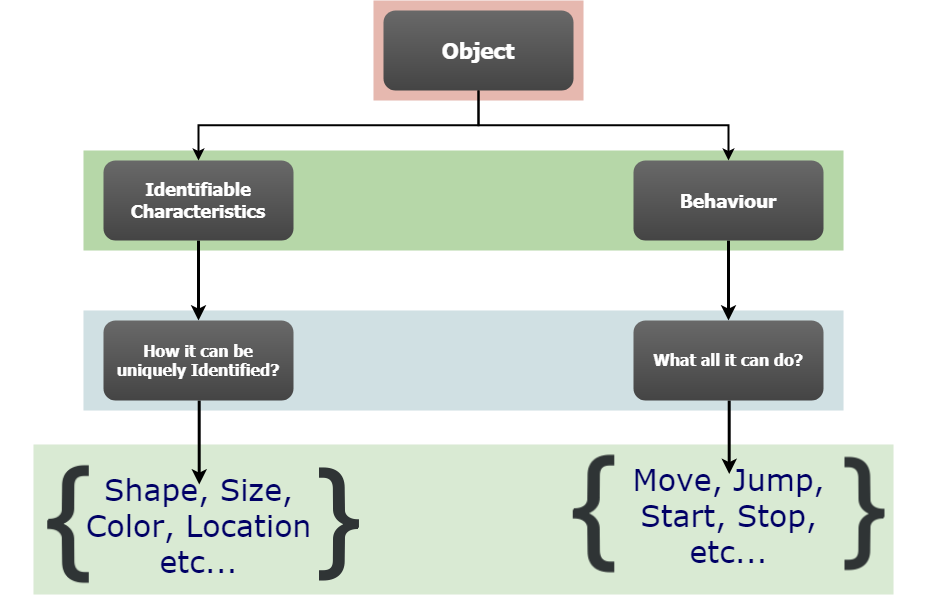
\includegraphics[width=1\textwidth, height=1\textheight, keepaspectratio]{./imgs/class_data_and_behaviour.png}
	\caption{Dati e comportamenti di una classe}
	\label{fig:class_data_and_behaviour}
\end{figure}

\textsf{\small Per creare una classe si utilizza la keyword \textbf{class}. Lo spazio di memoria non è allocata quando la classe viene definita, ma quando viene istanziata. } \\

\textsf{\small Per creare un'istanza della classe, si chiama il nome della classe e poi il nome dell'istanza.} \\

\subsection{Costruttori e Distruttori}

\subsubsection{Costruttori}

\textsf{\small \textbf{Definizione: } Il \textbf{costruttore} è una speciale funzione membro (della classe) che inizializza gli oggetti di una classe. Il costruttore è chiamato automaticamente quando un'istanza della classe viene creata. È una funzione speciale perché non tipi di ritorno, o meglio il tipo di ritorno è la classe stessa. } \\ %Funzione membro o membra?

\textsf{\small Il nome di questa funzione \textbf{costruttore} è identico al nome della classe stessa.} \\

\textsf{\small Se non specifichiamo un \textbf{costruttore}, uno di default verrà creato dal compilatore (senza parametri e con il corpo della funzione vuoto).} \\

\subsubsection{Distruttori}

\textsf{\small \textbf{Definizione: } Il \textbf{distruttore}, come dice la parola, è una funzione membro della classe che viene invocata automaticamente quando un oggetto (istanza della classe) viene distrutto/eliminato. Il che significa che il distruttore è l'ultima funzione ad essere chiamata. } \\

\textsf{\small Per definire un \textbf{distruttore} si crea una funzione con lo stesso nome della classe, ma prima del nome deve essere accompagnata dal simbolo \textbf{~} (tilde).} \\

\subsubsection{Proprietà del distruttore}

\begin{itemize}
	\item \textsf{\small Il distruttore è invocato automaticamente quando gli oggetti sono distrutti.}
	\item \textsf{\small Non può essere dichiarato \textbf{static} o \textbf{const}.}
	\item \textsf{\small Il \textbf{distruttore} non ha argomenti.}
	\item \textsf{\small Non ha tipi di ritorno, nemmeno \textbf{void}.}
	\item \textsf{\small Un oggetto della classe con un distruttore non può diventare membro di una \textbf{union}.}
	\item \textsf{\small Un distruttore dovrebbe essere dichiarato nella sezione \textbf{public}.}
	\item \textsf{\small Il programmatore non può accedere all'indirizzo del \textbf{distruttore}.}
	%\item \textsf{\small }
\end{itemize}

\subsubsection{Quando viene chiamato il distruttore?}

\begin{itemize}
	\item \textsf{\small La funzione finisce.}
	\item \textsf{\small Il programma termina.}
	\item \textsf{\small Un blocco contenente le variabili cessa.}
	\item \textsf{\small Un operatore \textbf{delete} viene chiamato.}
\end{itemize}

\begin{lstlisting}
	class MyClass {
		// Costruttore
		MyClass(){
			// Corpo del costruttore.
		}
		// Distruttore
		~MyClass(){
			// Corpo del distruttore.
		}
	}
\end{lstlisting}

\subsection{Access modifiers}

\textsf{\small \textbf{Definizione: } Gli \textbf{Access Modifiers} in una classe sono usati per assegnare l'accessibilità ai membri della classe. Questo permette una importante feature della programmazione ad oggetti, ovvero la \textbf{Data Hiding} che permette di prevenire l'accesso diretto dei dati da parte delle funzioni del programma.} \\

\textsf{\small Ci sono 3 tipi di \textbf{access modifiers}:} \break

\begin{tabular}{|c|c|}
	\hline
	\textbf{Access Modifier} & \textbf{Definizione} \\
	\hline
	\textsf{\small \textbf{public}} & \textsf{\small accessibile a tutti.} \\
	\hline
	\textsf{\small \textbf{private}} & \textsf{\small accessibile solo all'interno della classe stessa.} \\
	\hline
	\textsf{\small \textbf{protected}} & \textsf{\small accessibile solo alla classe, alle sue sottoclassi (ereditarietà)} \\
	\textsf{\small } & \textsf{\small ed alle classi amiche (friend class).} \\
	\hline
\end{tabular}

\subsubsection{Incapsulamento}

\textsf{\small \textbf{Definizione: } L'\textbf{incapsulamento} è un concetto di programmazione ad oggetti che mette assieme i dati e le funzioni che manipolano i dati per mantenerli sicuri da interferenze esterne e da un uso improprio.} \\

\textsf{\small L'\textbf{incapsulamento} dei dati è un meccanismo di impacchetamento di dati e delle funzioni che li usano. } \\

\textsf{\small La \textbf{Data abstraction} è un meccanismo che espone solo le interfacce e nasconde  i dettagli dell'implementazione dall'utente.} \break

%TODO: qui fare un esempio concreto.

\begin{lstlisting}
	class Sommatore {
		// con public sono accessibili da tutti.
	  public:
		// Costruttore.
		Sommatore(int i = 0){ // i = 0 vuol dire che assegniamo un valore di default, casomai l'utente non voglia inserirne uno.
			totale = i;
		}
	
		// Interfaccia al mondo esterno.
		void aggiungiNumero(int numero){
			totale += numero;
		}
	
		// Interfaccia al mondo esterno.
		int getTotale(){
			return totale;
		}
	
	private:
		// Dati nascosti al mondo esterno.
		int totale;
	};

	int main(){
		Sommatore s;
		
		s.aggiungiNumero(3);
		s.aggiungiNumero(6);
		s.aggiungiNumero(9);
		
		std::cout << "Totale: " << s.getTotale() << std::endl; // Output: Totale: 18
		return 0;
	}
\end{lstlisting}

%TODO: operatore :: (due punti)

\subsection{scope resolution operator ::}

\textsf{\small L'operatore \textbf{scope resolution} indicato con i \textbf{::} (doppi due punti) può essere usato per definire delle funzioni della classe fuori dalla stessa.} \\

\textsf{\small Può essere usato per accedere ad una variabile globale quando c'è anche una variabile locale con lo stesso nome.} \\

\textsf{\small Può essere usato quando si ha la definizione di una classe all'interno di un'altra classe.} \\

\begin{lstlisting}
#include <iostream>
int weight = 33;
	
class MyClass {
	public:
		MyClass(){
			num = 66;
		}	
	
		void display();
		
		int get_num(){
			return num;
		}
	
	private:
		int num;
};

void MyClass::display(){
	std::cout << "Il valore di num e\': " << get_num() << std::endl;
}

int main(){
	int weight = 99;
	MyClass istanza;
	istanza.display(); // Output: Il valore di num è: 66
	
	std::cout << "Valore della variabile weight locale: " << weight << std::endl;
	std::cout << "Valore della variabile globale: " << ::weight << std::endl; 
	return 0;
}
\end{lstlisting}

\subsection{Getters \& Setters}

\textsf{\small Per via dell'incapsulamento, per poter recuperare (getter) o impostare (settare) le variabili private usufruiamo dei \textbf{getters \& setters} che sono due funzioni, una per recuperare il dato (getter) e l'altro per impostarlo (setter).} \\

\begin{lstlisting}
	class MyClass {
	public:
		MyClass(){
			// Costruttore
		}
	
		// Recupera il valore della variabile number.
		int get_number(){
			return number;
		}
		
		// Imposta un nuovo valore alla variabile number.
		void set_number(int number_t){
			number = number_t;
		}
	
	private:
		int number;
	};
\end{lstlisting}

\subsection{Ereditarietà}

\textsf{\small \textbf{Definizione: } L'\textbf{ereditarietà} è la capacità di derivare le proprietà e le caratteristiche da un'altra classe. È una delle feature più importanti della programmazione ad oggetti.} \\

\textsf{\small La classe che deriva è chiamata \textbf{derived class} o \textbf{sub class}, mentre quella che viene derivata è chiamata \textbf{base class} o \textbf{super class}.} \\

\textsf{\small Per implementare l'ereditarietà usiamo l'operatore \textbf{:} quando andiamo a definire la classe derivata. Questa è chiamata la \textbf{initialization list} serve per chiamare la classe base e per inizializzare le variabili membri prima che il costruttore venga eseguito.} \\

\begin{lstlisting}
	class nome_classe_derivata : modalità_di_accesso nome_classe_base {
		// Corpo della subclass/ derived class
	}
\end{lstlisting}

\begin{figure}[ht]
	\centering
	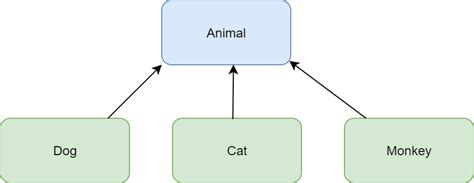
\includegraphics[width=1\textwidth, height=1\textheight, keepaspectratio]{./imgs/animal_class_uml.jpg}
	\caption{Concetto dell'ereditarietà}
	\label{fig:ereditarietà2}
\end{figure}

%TODO: aggiungere classe Monkey
\begin{lstlisting} 
	class Animal {
	public:
		Animal(){
			std::cout << "Animal Constructor" << std::endl;
		}
	
		void eat(){
			std::cout << "gnam gnam.." << std::endl;
		}
	
		void sleep(){
			std::cout << "Sleeping zzz.." << std::endl;
		}
	};

	class Dog : public Animal {
	public:
		Dog(std::string name, int weight){
			std::cout << "Dog Constructor" << std::endl;
			// Qui stiamo assegnando i valori dei parametri alle nostre variabili nella classe (quelle in private).
			// Per evitare confusioni potremmo anche chiamare i parametri del costruttore in maniera diversa (tipo: nomeparametro\_t per differenziarlo oppure \_nomeparametro) oppure per differenziare le variabili della classe potremmo aggiungerci la keyword this.
			name = name;
			weight = weight;
		}
	
		void bark(){
			std::cout << "Wuuf Wuuf" << std::endl;
		}
	
		std::string get_name(){
			return name;
		}
	
		int get_weight(){
			return weight;
		}
	
	private:
		std::string name;
		int weight;
	};

	class Cat : public Animal {
		public:
		Cat(std::string name, int weight){
			std::cout << "Cat Constructor" << std::endl;
			// Qui usiamo il puntatore this per far riferimento alle variabili membre della classe al posto di quelle passate come parametro al costruttore.
			this->name = name;
			this->weight = weight;
		}
		
		void meow(){
			std::cout << "Meow Meow" << std::endl;
		}
	
		std::string get_name(){
			return name;
		}
		
		int get_weight(){
			return weight;
		}
		
		private:
		std::string name;
		int weight;
	};

	int main(){
		Dog floki {"floki", 36};
		std::cout << floki.bark() << std::endl;
		std::cout << floki.get_name() << std::endl;
		std::cout << floki.get_weight() << std::endl;
		
		// Output: Animal Constructor
		// Output: Dog Constructor
		// Output: floki
		// Output: 36
		return 0;
	}
\end{lstlisting}

\begin{figure}[ht]
	\centering
	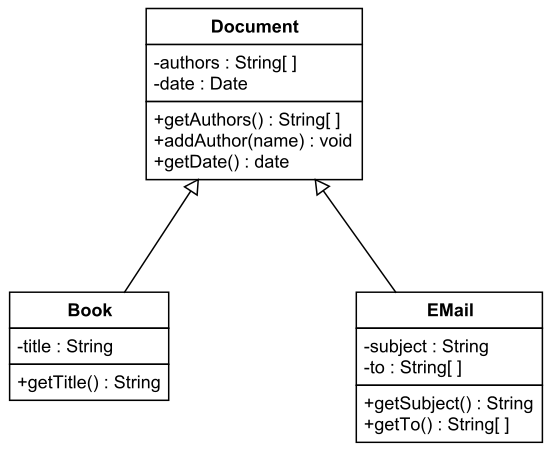
\includegraphics[width=1\textwidth, height=1\textheight, keepaspectratio]{./imgs/inheritance_class_uml2.jpg}
	\caption{Ereditarietà in un diagramma UML}
	\label{fig:ereditarietà}
\end{figure}

\subsubsection{this pointer}

\textsf{\small \textbf{Definizione: } La keyword \textbf{this} serve per riferirsi all'oggetto in cui ci troviamo.} \\ %TODO: da rivedere, aggiungere esempio, ecc..

\subsection{Multi-Ereditarietà}

%TODO: diamond problem: ambiguity, classe che deriva da due classi che entrambe derivano dalla stessa base class?

\textsf{\small Il c++ permette l'\textbf{ereditarietà multipla}, quindi una classe può derivare da più classi base. Non è presente invece l'implementazione di interfacce.} \\

\begin{lstlisting}
	class A
	{
		public:
		A()  { cout << "A's constructor called" << endl; }
	};
	
	class B
	{
		public:
		B()  { cout << "B's constructor called" << endl; }
	};
	
	class C: public B, public A  // Da notare l'ordine.
	{
		public:
		C()  { cout << "C's constructor called" << endl; }
	};
	
	int main()
	{
		C c;
		// Output: B's constructor called
		// Output: A's constructor called
		// Output: C's constructor called
		return 0;
	}
\end{lstlisting}

\subsection{Forward Declaration}

\textsf{\small \textbf{Definizione: } La \textbf{forward declaration} è quando prima dichiariamo una funzione, una classe, eccetera.. con la premessa che da qualche parte nel codice più in là ci sarà una definizione di questa funzione, classe, eccetera..} \\

\textsf{\small Può essere utile per aiutare il compilatore per assicurarsi che non ci sono stati errori di spelling o di numero sbagliato di argomenti da passare.} 

\textsf{\small Può essere utile per ridurre il tempo di \emph{build} del programma.}

\textsf{\small Può essere utile per rompere il ciclo delle referenze dove due definizioni si usano a vicenda.} \\

\begin{figure}[H]
	\centering
	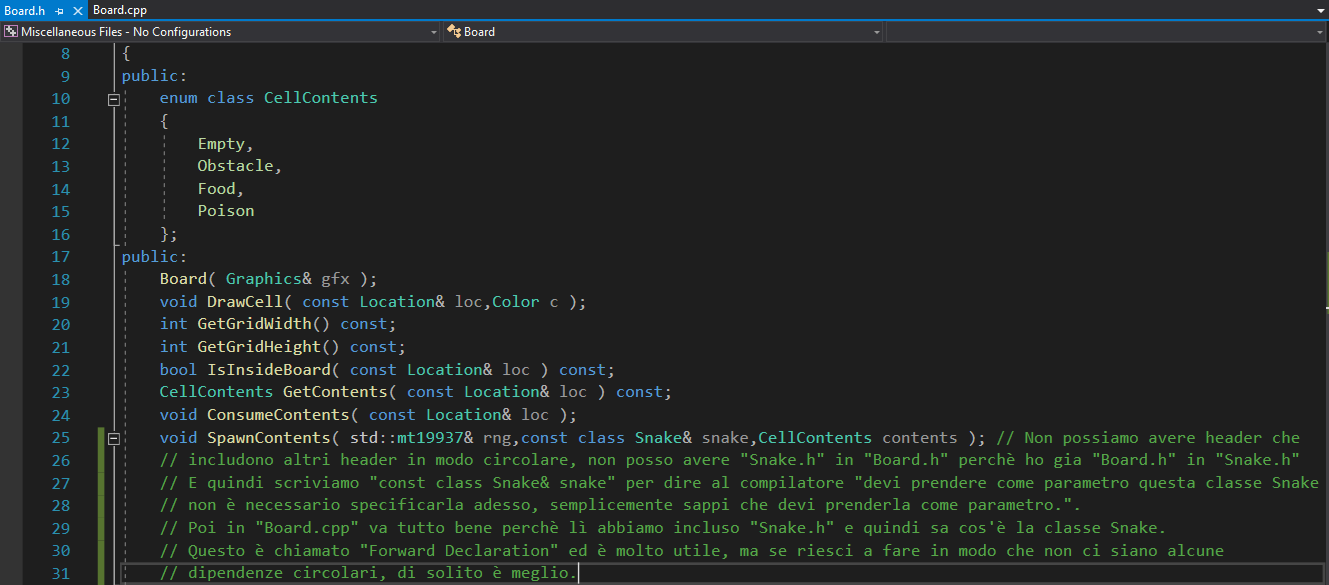
\includegraphics[width=1.2\textwidth, height=1.2\textheight, keepaspectratio]{./imgs/Forward_declaration.png}
	\caption{Forward Declaration}
	\label{fig:forward_declaration}
\end{figure}

%TODO: aggiungere il resto del codice dell'immagine potrebbe essere utile

\subsection{Chiamata a funzione statica e a membro} 

\subsubsection{Static nelle Classi}

\textsf{\small \textbf{Definizione: } Possiamo definire un membro della classe statica attraverso la keyword \textbf{static}. Questo significa che non importa quante istanze della classe vengano create, c'è una sola copia del membro statico.}

\textsf{\small Un membro statico è condiviso da tutti gli oggetti della classe. Se non è presente un'inizializzazione al membro statico, il suo valore di default sarà 0.} \\ 

\textsf{\small Per accedere a questa funzione statica o membro o altro \textbf{non} possiamo utilizzare l'operatore \textbf{.}, ma dobbiamo usufruire dell'operatore \textbf{::}.} \\

\begin{lstlisting}
class MyClass {
	public:
		MyClass(){
			// Costruttore
		}	
	
		// Questo è un esempio, non ho messo l'implementazione della funzione.
		static int calcola_qualcosa() {};
};

int main(){
	MyClass oggetto;
	// Non posso fare oggetto.calcolaQualcosa();
	// Devo fare MyClass::calcola\_qualcosa();
	MyClass::calcola_qualcosa();
	return 0;
}
\end{lstlisting}

\begin{figure}[H]
	\centering
	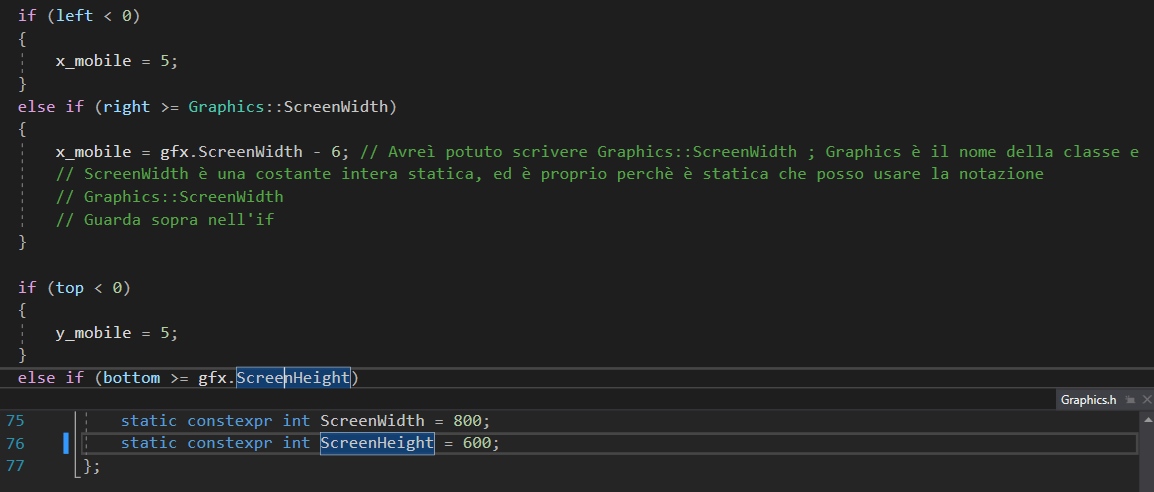
\includegraphics[width=1.2\textwidth, height=1.2\textheight, keepaspectratio]{./imgs/Class__static_type2.png}
	\caption{Chiamata a membro statico}
	\label{fig:class_static_type}
\end{figure}

\subsection{Funzioni e la keyword const}

\textsf{\small Ci sono vari significati che la keyword \textbf{const} assume e fa assumere alla funzione quando si trova in essa.} \\

\textsf{\small Mettendo \textbf{const} nei parametri della funzione, ciò significa che i parametri di quella funzione non possono essere cambiati, perché sono costanti.}

%TODO: esempio

%TODO: const come return type.

\begin{figure}[H]
	\centering
	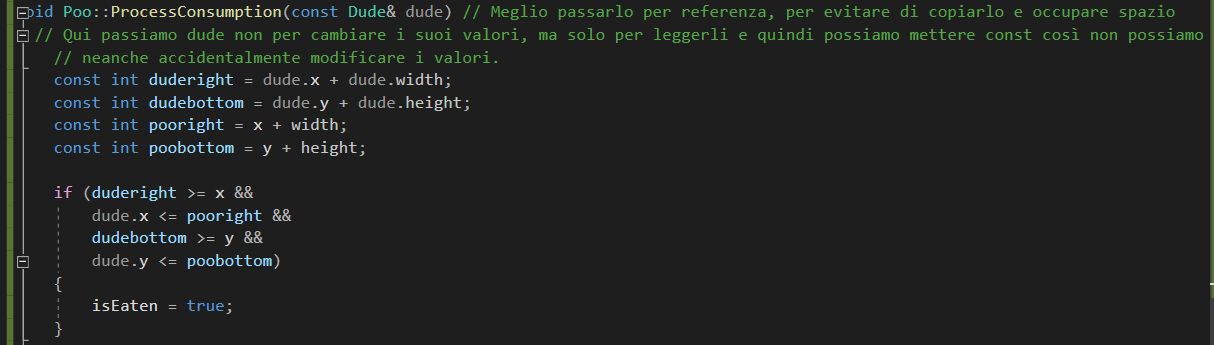
\includegraphics[width=1.2\textwidth, height=1.2\textheight, keepaspectratio]{./imgs/const_as_parameter.png}
	\caption{Const come parametro}
	\label{fig:const_as_parameter}
\end{figure}

\textsf{\small Mentre, la keyword \textbf{const} alla fine della funzione (Const member function in inglese) significa che l'oggetto chiamato da questa funzione non può essere modificato, questo previene modifiche accidentali all'oggetto. } \\

\begin{lstlisting}
	int val = 5;
	
	// Se aggiungessimo una riga per modificare il valore, otterremmo un errore.
	// Inoltre mettere quel const lì esprime l'intento di non cambiare l'oggetto 
	// della funzione.
	int getValue() const
	{
		return val;
	}
\end{lstlisting}

\begin{figure}[H]
	\centering
	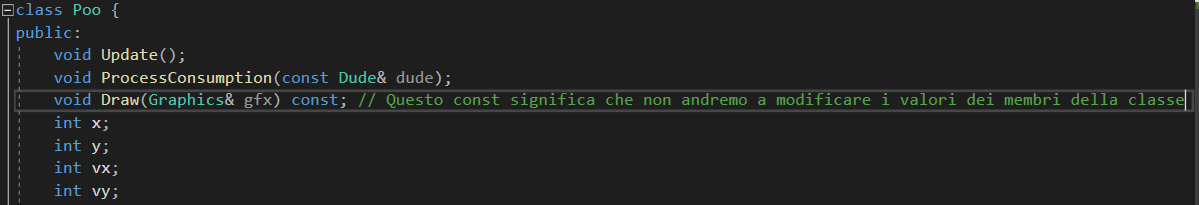
\includegraphics[width=1.2\textwidth, height=1.2\textheight, keepaspectratio]{./imgs/const_function_class_members.png}
	\caption{Const function class members}
	\label{fig:const_function_class_members}
\end{figure}

\textsf{\small Infine, c'è restituire \textbf{const} come valore di ritorno di una funzione, ma non sembra di molta utilità, tranne per le move-semantics, per lo meno se lo si ritorna per valore, mentre ritornarlo per reference protegge il valore di ritorno dall'essere modificato.} \\

\subsection{Class vs Struct}

\textsf{\small In C++ le classi e le strutture sono simili, ma con alcune differenze:} \break

\begin{tabular}{|c|c|}
	\hline
	\textbf{Class} & \textbf{Struct} \\
	\hline
	\textsf{\small I membri della classe sono privati da default.} & \textsf{\small I membri di una struttura sono pubblici da default.} \\
	\hline
	\textsf{\small L'allocazione della memoria avviene nell'heap.} & \textsf{\small L'allocazione della memoria avviene sullo stack.} \\
	\hline
	\textsf{\small È un tipo di dato per referenza.} & \textsf{\small È un tipo di dato per valore.} \\
	\hline
	\textsf{\small Si dichiara usando la keyword \textbf{class}.} & \textsf{\small Si dichiara usando la keyword \textbf{struct}.} \\
	\hline
	%\textsf{\small } & \textsf{\small } \\
\end{tabular}

%TODO: costruttori, distruttori, copy, move, rule of 3, rule of 5. (rule of 7?); Forse alcune cose in un altro capitolo. (queste assieme al polimorfismo nel secondo capitolo).

%TODO: non usare la keyword new per istanziare?! e delete, magari subsections sulla new e la delete.

% -------------------------- SECTION: OPERATORS --------------------------------------

%\section{Operators}

%TODO: come creare operatori, però questo potrei metterlo in un altro capitolo, non qui nelle basi del linguaggio.

%TODO: aggiungere le Convenzioni del linguaggio.

% -------------------------- SECTION: CONVENZIONI ------------------------------------

\newpage

\section{Convenzioni del linguaggio}

\textsf{\small \textbf{Definizione: } Le \textbf{convenzioni} sono delle linee guida di un linguaggio che raccomandano un certo stile di programmazione. Queste permettono un codice più chiaro, più leggibile e rende il codice di un software più semplice da mantenere.} \\

\textsf{\small Inoltre, sia il codice che i commenti dovrebbero essere in inglese a differenza di come ho fatto io in questa guida.} \\

\textsf{\small Potete trovare tutte le convenzioni del linguaggio nelle \textbf{C++ Core Guidelines} : \href{https://github.com/isocpp/CppCoreGuidelines}{CppCoreGuidelines}} \\

\textsf{\small Qui anche una versione più corta (non ufficiale): \href{https://github.com/openbmc/docs/blob/master/cpp-style-and-conventions.md}{CppStyleAndConventions}} \\

\textsf{\small Comunque ne elencherò qualche d'una: } \break

\subsection{Generale}

\begin{itemize}
	\item \textsf{\small Lunghezza della riga limitata a 80 caratteri}
	\item \textsf{\small Indentazione con 4 spazi.}
	\item \textsf{\small I files dovrebbero usare le newlines stile Unix $\backslash n$.}
\end{itemize}

\subsection{Parentesi Graffe}

\textsf{\small Utilizzare \emph{Allman Style} brackets (parentesi). Le parentesi graffe sono sulla loro linea allo stesso livello con lo statement sopra.} \\

\begin{lstlisting}
	if (condition)
	{
	
	}
\end{lstlisting}

\textsf{\small Anche gli if con una sola linea dovrebbero avere le parentesi graffe.} \\

\subsection{Indentazione}

\textsf{\small Il contenuto in un \textbf{namespace} dovrebbe essere allo stesso livello di indentazione del namespace stesso. } \\

\textsf{\small Il contenuto in una \textbf{classe}, \textbf{struct}, \textbf{funzioni}, \textbf{if}, \textbf{loop}, \textbf{switch}, \textbf{cases} e \textbf{labels} (dei goto) dovrebbe essere indentato.} \\

\subsection{Convenzioni sui nomi}

\begin{itemize}
	\item \textsf{\small Non c'è nè prefisso nè suffisso a nessun nome.}
	\item \textsf{\small Gli acronimi dovrebbero essere dello stesso case.}
\end{itemize}

\begin{lstlisting}
	// Correct.
	SomeBMCType someBMCVariable = bmcFunction();
\end{lstlisting}

\subsection{Ordine Inclusione Header files}

\textsf{\small Inclusione degli headers in un header file:} \\

\begin{itemize}
	\item \textsf{\small headers locali}
	\item \textsf{\small librerie c}
	\item \textsf{\small librerie cpp}
\end{itemize}

\textsf{\small Inclusione degli headers in un source file (.cpp):} \\

\begin{itemize}
	\item \textsf{\small source.hpp (se applicabile)}
	\item \textsf{\small headers locali}
	\item \textsf{\small librerie c}
	\item \textsf{\small librerie cpp}
\end{itemize}

\textsf{\small In ordine alfabetico.} \\

\subsubsection{Files}

\begin{itemize}
	\item \textsf{\small Gli headers C++ dovrebbero finire in \emph{.hpp}. Gli headers C dovrebbero finire in \emph{.h}.}
	\item \textsf{\small I files dovrebbero essere chiamati nel modo (case) lower\_snake\_case.}
\end{itemize}

\subsection{Types}

\begin{itemize}
	\item \textsf{\small Preferire \emph{using} a \emph{typedef}.}
	\item \textsf{\small Le strutture, classi, enums dovrebbero essere tutti in UpperCamelCase.}
	\item \textsf{\small Preferire gli scope namespaces al posto di nomi con lunghi prefissi.}
	\item \textsf{\small Un alias di una singola parola con una struct / class dovrebbe essere in minuscolo, ma un alias a più parole dovrebbe essere UpperCamelCase.}
	\item \textsf{\small Eccezioni: Una libreria API potrebbe usare il modo lower\_snake\_case per accordarsi alle convenzioni STL o ad una libreria C. Application APIs dovrebbero tutte essere UpperCamelCase.}
	\item \textsf{\small Eccezione: Per convenienza un tipo di una classe template potrebbe finire in \_t per accordarsi alle convenzioni STL.}
	%\item \textsf{\small }
\end{itemize}

\subsection{Variabili}

\textsf{\small Le variabili dovrebbero tutte essere lowerCamelCase, inclusi i membri delle classi, senza underscore (trattini bassi).} \\

\subsection{Funzioni}

\begin{itemize}
	\item \textsf{\small Le funzioni dovrebbero essere lowerCamelCase.}
	\item \textsf{\small Eccezione: Una libreria API potrebbe usare lower\_snake\_case in accordo con le convenzioni STL o di una sottostante libreria in C che sta astraendo. Application API dovrebbero tutte essere lowerCamelCase.}
	%\item \textsf{\small }
\end{itemize}

\subsection{Costanti}

\begin{itemize}
	\item \textsf{\small Costanti e i membri delle enums dovrebbero essere chiamati come le variabili in lowerCamelCase.}
\end{itemize}

\subsection{Namespaces}

\begin{itemize}
	\item \textsf{\small I namespaces dovrebbero essere lower\_snake\_case.}
	\item \textsf{\small Top-level namespace dovrebbe essere chiamato sulla base della repository che lo contiene.}
	\item \textsf{\small Favorisci un namespace chiamato 'details' o 'internal' per indicare l'equivalente di un namespace 'private' in un header file e namespaces anonimi in un file C++.}
\end{itemize}

\subsection{Header Guards}

\textsf{\small Preferire \textbf{\#pragma} allo stile \textbf{\#ifndef}.}\\

\subsection{Spazi bianchi addizionali}

\begin{itemize}
	\item \textsf{\small Segui lo stile di dichiarazione del C++}
\end{itemize}

\begin{lstlisting}
	foo(T& bar, const S* baz); // Correct.
	foo(T &bar, const S *baz); // Incorrect.
\end{lstlisting}

\begin{itemize}
	\item \textsf{\small Usa gli spazi bianchi moderatamente.}
	\item \textsf{\small Inserisci uno spazio bianco prima e dopo if e loops.}
\end{itemize}

\begin{lstlisting}
	if (...)
	while (...)
	for (...)
\end{lstlisting}

\begin{itemize}
	\item \textsf{\small Aggiungi spazio bianco attorno agli operatori binari per leggibilità}
\end{itemize}

\begin{lstlisting}
	foo((a-1)/b,c-2); /// Incorrect.
	foo((a - 1) / b, c - 2); /// Correct.
\end{lstlisting}

\begin{itemize}
	\item \textsf{\small Non inserire spazi bianchi dopo gli operatori unari.}
\end{itemize}

\begin{lstlisting}
	a = * b;  /// Incorrect.
	a = & b;  /// Incorrect.
	a = b -> c;  /// Incorrect.
	if (! a)  /// Incorrect.
\end{lstlisting}

\begin{itemize}
	\item \textsf{\small Non inserire spazi bianchi nè prima nè dopo una chiamata a funzione e ai parametri.}
\end{itemize}

\begin{lstlisting}
	foo(x, y); /// Correct.
	foo ( x , y ); /// Incorrect.
	
	do (...)
	{
	} while(0); /// 'while' qui è strutturato come una chiamata a funzione.
\end{lstlisting}

\begin{itemize}
	\item \textsf{\small Preferire una linea a capo dopo gli operatori per mostrare la continuazione.}
\end{itemize}

\begin{lstlisting}
	if (this1 == that1 &&
	this2 == that2) /// Correct.
	
	if (this1 == that1
	&& this2 == that2) /// Incorrect.
\end{lstlisting}

\begin{itemize}
	\item \textsf{\small Le linee lunghe dovrebbero avere la continuazione che inizi allo stesso livello delle parentesi o tutti gli oggetti all'interno delle parentesi dovrebbero essere al secondo livello di indentazione.}
\end{itemize}

\begin{lstlisting}
	reallyLongFunctionCall(foo,
	bar,
	baz); // Correct.
	
	reallyLongFunctionCall(
	foo,
	bar,
	baz); // Also correct.
	
	reallyLongFunctionCall(
	foo, bar, baz); // Similarly correct.
	
	reallyLongFunctionCall(foo,
	bar,
	baz); // Incorrect.
\end{lstlisting}

\subsection{Linee Guida Miste}

\begin{itemize}
	\item \textsf{\small  Usare sempre size\_t o ssize\_t per cose come contatori, pesi, ecc.. C'è bisogno di un forte motivo razionale per usare un tipo come uint8\_t quando size\_t può fare lo stesso lavoro.}
	\item \textsf{\small Usa uint8\_t, int16\_t, uint32\_t, int64\_t quando è importante per l'interazione coll'hardware. Non usarli senza una buona motivazione, quando le interazioni coll'hardware non sono coinvolte; preferire size\_t o int piuttosto.}
\end{itemize}

% ------------------------- PER ALTRI CAPITOLI ---------------------------------------

%TODO: lambdas, ma non in questo capitolo.
%TODO: operazioni su file
%TODO: elissi.

%TODO: inline functions
%TODO: this Pointer
%TODO: Pointer to Class
%TODO: Static member of class
%TODO: friend functions
%TODO: virtual keyword
%TODO: Multi-Inheritance, ma non le interfacce. (forse qui o forse no)
%TODO: Destructors call order. (in un altro capitolo)
% Nome sezione: Approfondimenti sulle Classi oppure Classi Concetti intermedi.

%TODO: diamond problem: ambiguity, classe che deriva da due classi che entrambe derivano dalla stessa base class.

%TODO: abstract class
%TODO: decltype